\documentclass[sort&compress, preprint]{elsarticle}
\usepackage[english]{babel}
\usepackage{amsmath,amssymb}
\usepackage{amsthm}
\usepackage{mathabx}
\usepackage{thmtools, thm-restate}
\usepackage{breqn}
\usepackage{bbold}
\usepackage{booktabs}
\usepackage{graphicx}
\usepackage[utf8]{inputenc}
\usepackage[T1]{fontenc}
\usepackage{caption}
\usepackage{siunitx}
\usepackage{hyperref}
\usepackage[labelfont=bf,textfont={sl,bf},lofdepth,lotdepth]{subfig}
\usepackage{xspace}
\usepackage{color}
\usepackage{proba}
\usepackage[usenames,dvipsnames,svgnames,table]{xcolor}
\usepackage{cleveref}
\usepackage{paralist}
\usepackage{todonotes}
\usepackage{bigints}
\usepackage[title,titletoc,toc]{appendix}
\usepackage{import}
\usepackage{natbib}
%%%%%%%%%%%%%%%%%%%%%%%%%%%%%%%%%%%%%%%%%%%%%%%%%%%%%%%%%%%%%%%%%%%%%%%%%%%%%%%%%%%%%%%%%%
%                                  MODIFICACIONES                                        %
%%%%%%%%%%%%%%%%%%%%%%%%%%%%%%%%%%%%%%%%%%%%%%%%%%%%%%%%%%%%%%%%%%%%%%%%%%%%%%%%%%%%%%%%%%
\oddsidemargin=1.0cm
%\evensidemargin=2.0cm
\textwidth=14.5cm
%%%%%%%%%%%%%%%%%%%%%%%%%%%%%%%%%%%%%%%%%%%%%%%%%%%%%%%%%%%%%%%%%%%%%%%%%%%%%%%%%%%%%%%%%%
%                                 FORMATOS                                               %
%%%%%%%%%%%%%%%%%%%%%%%%%%%%%%%%%%%%%%%%%%%%%%%%%%%%%%%%%%%%%%%%%%%%%%%%%%%%%%%%%%%%%%%%%%
%\DeclareMathAlphabet{\mathpzc}{OT1}{pzc}{m}{it}
\theoremstyle{definition}
\newtheorem{definition}{Definition}[section]
\newtheorem{dfn}{Definition}[section]
\newtheorem{assumption}{Assumption}[section]
\newtheorem{hypothesis}{Hypothesis}[section]
%
\theoremstyle{plain}% default
\newtheorem{thm}{Theorem}[section]
\newtheorem{pro}{Proposition}[section]
\newtheorem{lem}{Lemma}[section]
\newtheorem{corollary}{Corollary}[section]
\newtheorem{consequence}{CONSEQUENCE}[section]
\newtheorem{example}{\bf Example}[section]
\theoremstyle{remark}
\newtheorem{remark}{Remark}[section]
\newproof{pf}{Proof}

%declaration theorems for appendix
\declaretheorem[numbered=no, name=H\"{o}lder]{Holder}
\declaretheorem[numbered=no, name=Young]{Young}
\declaretheorem[numbered=no, name=Minkowski]{Minkowski}
\declaretheorem[numbered=no, name=Doob's Martingale Inequality]{Doobs}
\declaretheorem[numbered=no, name=Burkholder–Davis–Gundy inequality]{bdg}
\declaretheorem[numbered=no, name=Gronwall inequality]{Gronwall}
\declaretheorem[numbered=no, name=Discrete Gronwall Inequality]{DiscreteGronwall}
\declaretheorem[numbered=no, name=A standard inequality]{Standard}
%
\providecommand*{\lemautorefname}{Lemma}
\providecommand*{\thmautorefname}{Theorem}
\providecommand*{\assumptionautorefname}{Assumption}
\providecommand*{\hypothesisautorefname}{Hypothesis}
\newcommand{\normL}[1]{\left[\mathbb{E}\left|#1\right|^2\right]^{1/2}}
\newcommand{\ms}[1]{\mathbb{E}\left|#1\right|^2}
\newcommand{\mep}[1]{\mathbb{E}|#1|^p}
\newcommand{\m}[1]{\mathbb{E}#1}
\newcommand{\Prob}[1]{\mathbb{P}\left[#1\right]}
\newcommand{\meanp}[2]{\mathbb{E}\left|#1\right|^{#2}}
\newcommand{\condexp}[2]{\mathbb{E}\left[#1|#2\right]}
\newcommand{\lftrght}[3]{\left#2 #1\right #3}\DeclareMathOperator{\tr}{tr}
\newcommand{\innerprod}[2]{\left\langle#1, #2\right\rangle}
\newcommand*{\eg}{e.g.,\xspace}
\newcommand*{\ie}{i.e.,\xspace}
\newcommand{\overbar}[1]{\mkern 1.5mu\overline{\mkern-1.5mu#1\mkern-1.5mu}\mkern 1.5mu}

%\newcommand*{\todo}[1]{\textcolor{BrickRed}{#1}\\}
\newcommand{\crefrangeconjunction}{--}
\crefrangeformat{equation}{(#3#1#4)--(#5#2#6)}
\DeclareMathOperator{\diag}{diag}
\DeclareMathOperator*{\as}{a.s.}
%\DeclareMathOperator{\diag}{diag}
\newcommand{\SM}{LS\xspace}
\AtBeginDocument{\renewcommand{\harvardand}{and}}
\declaretheorem[numberwithin=section]{theorem}
\crefname{hypothesis}{hypothesis}{hypotheses}
\Crefname{hypothesis}{Hypothesis}{Hypotheses}
%opening
\begin{document}
	\begin{frontmatter}
		\title{
				Strong Convergence and Almost Sure Stability of the Explicit Linear Steklov Method
				for SDEs under non-globally Lipschitz Coefficients.\tnoteref{t1}
		}%,t2}}
		\tnotetext[t1]{
			This work has been partially
			supported by CONACYT project *****
		}
		\author[sj]{S. D\'{\i}az-Infante}
		\ead{sauld@cimat.mx}
		\author[sj]{S. Jerez}
		\ead{jerez@cimat.mx}
		\address[sj]{Split Step Linear Steklov Method 
		Department of Applied Mathematics, CIMAT, Guanajuato, Gto., Mexico,
		36240.
		}
	\begin{abstract}
		We present an explicit and easily implementable numerical method for
		solving stochastic differential equations (SDEs) with non-globally Lipschitz
		coefficients. A linear version of the Steklov average under a split-step formulation supports our new solver.
		The Linear Steklov (\SM) method converges strongly with a standard 
		one-half order.  Also, we study the almost sure asymptotic stability and to emphasize his 
		performance we use models from population dynamics and non linear stochastic oscillators.
	\end{abstract}
	\begin{keyword}
		stochastic differential equations;
		explicit methods; strong convergence; almost surely asymptotic stability.
	\end{keyword}
	\end{frontmatter}
	\pagebreak
	\tableofcontents
	\pagebreak
	%\import{papers/paperB/sections/}{abstract.tex}
	\section{Introduction}
		%	Applications of Monte Carlo type simulations \cite{Glasserman2004,Giles2008} as  Brownian Dynamics \cite{Cruz2012}
%require  fast numerical methods with low computational cost --- excluding the use of 
%implicit schemes in the majority of cases.
%The EM method is the most popular in such  
%simulations due to its simple algebraic structure, cheap computational cost and acceptable convergence rate 
%under global Lipschitz conditions. 
%However, if the drift or diffusion coefficient of stochastic 
%differential equation  is super-linear, then the EM approximation 
%diverges  in the mean square sense \cite{Hutzenthaler2009, Hutzenthaler2012b}. 
%In most applications, the coefficients of the stochastic  models in finances, biology or physics 
%have locally Lipschitz coefficients with super-linear growth. 
%Therefore, recent research has been focused on modifying the EM method to obtain strong convergence  under these 
%conditions keeping its simple structure and  its low computational cost. In the last years, 
%several methods have been developed in this direction:  the family of  Tamed schemes
%\cite{Hutzenthaler2012a, Wang2011, Zong2014,Hutzenthaler2015,Sabanis2015}, 
%a special type of balanced method \cite{Tretyakov2013},  the stopped scheme \cite{Liu2013a} and 
%a truncated Euler method  \cite{Mao2015}.
%In these works, the strong convergence of the proposed method
%is proved using the theory developed by Higham, Stuart and 
%Mao in \cite{Higham2002b} or by means of  the new approach given by  Hutzenthaler and Jentzen in 
%\cite{Hutzenthaler2015}.
%Both techniques obtain the property of  strong convergence by proving boundedness moments of the numerical and 
%analytical solution of the underlying SDE. In spite of the recent work in this subject,  it is still necessary
%to get more accurate numerical methods for SDE under super-linear growth and 
%non-globally Lipschitz coefficients.

	In this chapter, we develop an explicit method based on a linear version  of the Steklov method proposed 
in  \Cref{ch:Chapter3}. We consider the vector It\^o stochastic differential equation
\begin{equation}\label{eqn:SDE1}
	dy(t)
	 =f(y(t))dt + g(y(t))dW(t), \quad 0\leq t\leq T,
	\quad y(0)=y_0,
\end{equation}
where $(f^{(1)},\dots, f^{(d)}):\R^d \to \R^d$ is one sided Lipschitz and 
$g = (g^{(j,i)})_{j\in \{1,\dots,d\}, i\in\{1,\dots, m\}}:\R^d \to \R^{d\times m}$ is global Lipschitz. 
Also we assume 
that  each component function $f^{(j)}$  can be written of the form
\begin{equation}\label{eqn:AlternativeConstruction}
	f^{(j)}(x) = a_j(x) x^{(j)} + b_j (x^{(-j)}), 
\end{equation}
where $a_j$ and	$b_{j}$ are two scalar 	functions in  $\R^d$ 
and $x^{(-j)} = \left( x^{(1)},\dots,x^{(j-1)},x^{(j+1)},\dots x^{(d)}\right)$.%
	\section{General Settings}
		
Throughout this paper, 
we work with a standard setup, that is,  $y(t)\in \R^d$ for each 
$t$ and  $W(t)$ is a
$m$-dimensional standard Brownian motion on a filtered and complete probability space
$	(
		\Omega ,\calF,(\calF_t)_{t\in[0,T]},\prob{}
	)$,
with the filtration
$(\mathcal{F}_t)_{t\in[0,T]}$  generated by the Brownian process.  Moreover,
we denote  the norm of a vector $y\in \R^d$ and the Frobenious norm 
of a matrix $G\in \R^{d\times m}$  by $|y|$ and $|G|$ respectively. The usual scalar product of two vectors 
$x,y\in \R^d$ is denoted by $\innerprod{x}{y}$.  The complement of a set $E$ is denoted by $E^c$ and 
the indicator function  of the set $E$ is denoted by $\1{E}$. 
In the following, we recall some classical results  about the moment boundedness, existence 
and uniqueness of the solution of the stochastic differential system \eqref{eqn:SDE1}, 
see \cite{Higham2002b,Mao2013,Mao2007}. We  also state some theorems about the strong 
convergence of the Euler-Maruyama method given by Higham et al. in \cite{Higham2002b} which will be useful 
 to prove the strong convergence of the Linear Steklov method. 
 
Let us start by assuming the following:


	
\begin{hypothesis}\label[hypothesis]{ass:OSLC}
	The coefficients of SDE \eqref{eqn:SDE1} satisfy the conditions:
	\begin{enumerate}[({H}-1)]
		\item \label{ass:C1Functions}
		The functions $f,g$ are in the class $C^{1}(\R^d)$.
		\item
		\textbf{Local, global Lipschitz condition}. For each integer $n$, there is a positive
		constant $L_{f}=L_{f}(n)$ such that
		$$
		|f(u)-f(v)|^2 %\vee |g(x)-g(y)|^2
		\leq L_{f}|u-v|^2 \qquad \forall u,v \in \R^d, \qquad |u|\vee|v|\leq n,
		$$
		and there is a positive constant $L_g$ such that
		$$
		|g(u)-g(v)|^2 \leq L_{g}|u-v|^2,
		\qquad  \forall u,v \in \R^d.
		$$ 
		\item\label{ass:MonotoneCondition}
		\textbf{Monotone condition.} There exist two positive constants $\alpha$ and $\beta$
		such that
		\begin{equation}\label{eqn:MonotoneCondition}
		\innerprod{u}{f(u)} +\frac{1}{2}|g(u)|^2
		\leq \alpha +\beta |u|^2, \qquad \forall u \in \R^d.
		\end{equation}
	\end{enumerate}
\end{hypothesis}


Under \Cref{ass:OSLC} we can assure  existence and uniqueness 
of the solution of continuous system \eqref{eqn:SDE1}. Next we state  the bounds on the moments
 of the  solution of \eqref{eqn:SDE1}.
%
 \begin{thm}
 	Assume \Cref{ass:OSLC}  then for all $y(0)=y_0\in \mathbb{R}^d$   there exists a 
 	unique global solution $\{y(t)\}_{t\geq 0}$ to SDE \eqref{eqn:SDE1}. Moreover, the solution has the 
 	following properties for any $T>0$,
 	\begin{equation*}
 		\ms{y(T)}< 
 		\left(
 			|y_0|^2 +2\alpha T 
 		\right)e^{2\beta T},
 	\end{equation*}
 	and
 	\begin{equation*}
 	\Prob{\tau_n\leq T}
 	\leq \frac{
 		\left(
 		|y_0|^2 +2\alpha T 
 		\right)
 		e^{2\beta T}
 	}{n},
 	\end{equation*}
 	where $n$ is any positive integer and 
 	%\begin{equation*}
 	$\tau_n := \inf \{ t\geq 0 : |y(t)|>n\}$.
 	%\end{equation*}
 \end{thm}
% %
\begin{thm}
	\label{thm:MaoCoercive}
	Let $p\geq 2$ and $x_0\in L^p(\Omega, \mathbb{R}^d)$. Assume that there exits a constant $C>0$
	such that for all $(x,t)\in \mathbb{R}^d\times [t_0,T]$,
	\begin{equation*}
	\innerprod{x}{f(x,t)}+\frac{p-1}{2}|g(x,t)|^2 \leq C(1+|x|^2).
	\end{equation*}
	Then
	\begin{eqnarray*}
	\EX{\sup_{0\leq t \leq T}|y(t)|^p}&\leq& C \left(1+\mep{y_0}\right), \nonumber\\
	\m|y(t)|^p
	&\leq&
	2^{\frac{p-2}{2}}
	\left(
	1 + \m|y_0|^p
	\right)e^{Cpt}, \qquad \forall t\in[0,T].
	\end{eqnarray*}
\end{thm}
\begin{hypothesis}\label{ass:MomentBounds}
	The SDE \eqref{eqn:SDE1} the EM solution \eqref{eqn:EulerMaruyama} and its continuous extension 
	\eqref{eqn:EMContinuousExtension} satisfies
	\begin{equation*}
		\EX{
			\sup_{0\leq t\leq T}
			|y(t)|^p	
		}< \infty, \quad
	\EX{
		\sup_{0\leq k \leq N}
			|Y_k|^p	
	}< \infty, \quad
	\EX{
		\sup_{0\leq t\leq T}
		|\overline{Y}(t)|^p	
	} < \infty, \qquad \forall p\geq 1.
	\end{equation*}
\end{hypothesis}

%********************************************************************************************
%              Section 3
%********************************************************************************************


		%
\begin{thm}[{
		%\citeauthor{Mao2013}
	 \cite[Thm. 2.2]{Mao2013}}]
	Let \Cref{ass:OSLC} holds. Then for all $y(0)=y_0\in \mathbb{R}^d$ given, there exist a 
	unique global solution $\{y(t)\}_{t\geq 0}$ to SDE\eqref{eqn:SDE1}. Moreover, the solution has the 
	following properties for any $T>0$,
	\begin{equation*}
		\ms{y(T)}< 
		\left(
			|y_0|^2 +2\alpha T 
		\right)\exp(2\beta T),
	\end{equation*}
	and
	\begin{equation*}
	\Prob{\tau_n\leq T}
	\leq \frac{
		\left(
		|y_0|^2 +2\alpha T 
		\right)
		\exp(2\beta T)
	}{n},
	\end{equation*}
	where $n$ is any positive integer and 
	%\begin{equation*}
	$\tau_n := \inf \{ t\geq 0 : |y(t)|>n\}$.
	%\end{equation*}
\end{thm}
%
\begin{thm}[
		%\citeauthor{Mao2007} 
		{\cite[Thm. 2.4.1]{Mao2007}}
	]
	\label{thm:MaoCoercive}
	Let $p\geq 2$ and $x_0\in L^p(\Omega, \mathbb{R}^d)$. Assume that there exits a constant $C>0$
	such that for all $(x,t)\in \mathbb{R}^d\times [t_0,T]$,
	\begin{equation*}
	\innerprod{x}{f(x,t)}+\frac{p-1}{2}|g(x,t)|^2 \leq C(1+|x|^2).
	\end{equation*}
	Then
	\begin{equation*}
	\m|y(t)|^p
	\leq
	2^{\frac{p-2}{2}}
	\left(
	1 + \m|y_0|^p
	\right)\exp({Cpt}) \quad \text{ for all } t\in[0,T].
	\end{equation*}
\end{thm}
%
\begin{lem}[
	{
		%\citeauthor{Higham2002b}
		\cite[Lem 3.2]{Higham2002b}}
	]
	\label{lem:MomentBound}
	Under \Cref{ass:OSLC}, for each $p\geq 2$, there is a $C=C(p,T)$ such that
	\begin{equation*}
	\EX{\sup_{0\leq t \leq T}|y(t)|^p}\leq C \left(1+\mep{y_0}\right).
	\end{equation*}
\end{lem}
%
	\section{Construction of the Linear Steklov method}
		%
	For simplicity, we begin the construction of the Linear Steklov method (\SM) considering the scalar case of SDE 
\eqref{eqn:SDE1}, that is, when $d=m=1$, also, to shorten notation we use $a,b$ instead $a_j,b_j$. 
Tough this ideas, we will generalize to higher dimensions.
Let $0=t_0 < t_1< \cdots < t_N=T$ a partition of the interval $[0,T]$ with constant step-size $h=T/N$ and such that
$t_k=kh$ for $k=0,\ldots, N$. The main idea of the  \SM approximation  consists in 
estimating the drift coefficient of \eqref{eqn:SDE1}  by
\begin{equation}
	f(y(t)) \approx 
		\varphi_{f}(y(t_{\eta_{+}(t)})) =
		\left(
			\frac{1}{y(t_{\eta_+(t)})-y(t_{\eta (t)})}
			\bigint \limits
_				{y(t_{\eta(t)})}^{y(t_{\eta_+(t)})}
					\frac{du}
						{
							a(y(t_{\eta(t)}))u
							+b
						}
	\right)^{-1}, \qquad t\in [0,T],
\end{equation}
where
\begin{align*}
	\eta(t) &:=
	k\text{  for } t\in [t_k, t_{k+1}), \quad k\geq 0,\\
	\eta_{+}(t) &:= 
	k+1  \text{ for } t\in [t_k, t_{k+1}), \quad k\geq 0.
\end{align*}
So we define the \SM method for the scalar version of the SDE \eqref{eqn:SDE1} using a split-step formulation as follows
\begin{align}
	Y_k^{\star} &= Y_k + h \varphi_f(Y^{\star}_k), \label{eqn:SSLSM1}\\
	Y_{k+1}	&= Y_k^{\star} + g(Y_k^{\star})\Delta W_k \label{eqn:SSLSM2},
\end{align}
with $Y_0=y_0$ and  $\varphi_{f}\left(Y_k^{\star}\right)$ defined by 
\begin{equation}
	\varphi_{f}\left(Y_k^{\star}\right)
	=
		\left(
			\frac{1}{Y_{k}^{\star}-Y_{k}}
			\int 
			%\limits
			_{Y_{k}}^{Y_{k}^{\star}}
				\frac{du}
				{
					a(Y_k)u
					+b
				}
	\right)^{-1}
\end{equation}
This scheme combines a split-step technique with a linear version of an exact deterministic 
method see \cite{Diaz-Infante2015,Matus2005}. 
In detail, first we compute the discrete value $Y^{\star}_k$ using the Linear Steklov approximation \eqref{eqn:SSLSM1},
and next, $Y_{k+1}$ is obtained by adding the stochastic increment $g(Y_k^\star)\Delta W_k$.

	To higher dimensions, we adapt the same split step scheme \crefrange{eqn:SSLSM1}{eqn:SSLSM2} as follows. 
For each component equation $j\in\{1, \ldots,  d\}$, on the iteration $k\in\{1, \ldots,  N\}$ take
\begin{align}
	a_{j,k} &=
	a_j
	\left(
		Y^{(1)}_{k},
		\ldots, Y^{(d)}_{k}
	\right),
	&
	b_{j,k} =
	b_{j}
	\left(
			Y^{(-j)}_k
	\right).
\end{align}
So, define  
$
	\varphi_{f}(Y_k^{\star})=
		\left(
			\varphi_{f^{(1)}}(Y_k^{\star}),
			\ldots,
			\varphi_{f^{(d)}}(Y_k^{\star})
		\right)
$
by
\begin{equation}
	\varphi_{f^{(j)}}\left(Y_k^{\star}\right)
		=
		\left(
			\frac{1}{Y_{k}^{\star(j)}-Y_{k}^{(j)}}
			\int 
			%\limits
				_{Y_{k}^{(j)}}^{Y_{k}^{\star(j)}}
				\frac{du}
				{
					a_{j,k} u
					+b_{j,k}
				}
		\right)^{-1}.
\end{equation}
%
	It is worth mentioning that even this formulation is semi implicit, we always can derive a explicit version. 
The next result deals with this issue. To simplify notation, we define  $A^{(1)}= A^{(1)}(h,u)$,  $A^{(2)}=A^{(2)}(h,u)$  and $b=b(u)$ by 
\begin{align}\label{eqn:SolutionFunctions}	
	A^{(1)}&:=
		\begin{pmatrix}
			e^{ha_1(u)} & \multicolumn{2}{c}{\text{\kern0.5em\smash{\raisebox{-1ex}{\huge 0}}}} \\
			&\ddots\\
			\multicolumn{2}{c}{\text{\kern-0.5em\smash{\raisebox{0.95ex}{\huge 0}}}} 
			& e^{ha_d(u)}
		\end{pmatrix},
		\notag
		\\
		%	
	A^{(2)}&:=
	\begin{pmatrix}
		\left(
			\displaystyle
			\frac{e^{ha_1(u)} - 1}{a_1(u)}
		\right)\1{E_1^c}	& 
		\multicolumn{2}{c}{\text{\kern0.5em\smash{\raisebox{-1ex}{\huge 0}}}}\\
		 & \ddots&\\
		\multicolumn{2}{c}{\text{\kern0.5em\smash{\raisebox{-1ex}{\huge 0}}}}&
		\left(
			\displaystyle
			\frac{e^{ha_d(u)} - 1}{a_d(u)}
		\right)\1{E_d^c}% + h \1{E_i} 
	\end{pmatrix}
	+h
	\begin{pmatrix}
		\1{E_1} & \multicolumn{2}{c}{\text{\kern0.5em\smash{\raisebox{-1ex}{\huge 0}}}}\\
		&\ddots &\\
		\multicolumn{2}{c}{\text{\kern0.5em\smash{\raisebox{-1ex}{\huge 0}}}} &
		\1{E_d}
	\end{pmatrix},\\	
	E_j&:=\{x \in \R^d: a_j(x)=0\} , \qquad 
	b(u):= \left(
		b_1(u^{(-1)}), \dots , b_d(u^{(-d)})
	\right)^T.		
	\notag
\end{align}
	Also we will need the following results from \cite[Thm 2.1]{Lawlor2012}, \cite[Thm. 1]{FineAIandKass1966}.
The first theorem will help us  with the singularities of set $E_j$ in the case where all elements of this set
are limit points. 
\begin{thm}[Multivariate L'h\^{o}pital's Rule] \label{thm:Lawlor}
	Let $\mathcal{N}$ be a neighborhood in $\R^2$ containing a point $\mathbf{q}$ at which
	two differentiable functions $f:\mathcal{N}\to \R$ and $g:\mathcal{N}\to \R$ are zero.
	Set 
	$$
		C=\{x \in \mathcal{N}: f(x)=g(x)=0 \},
	$$
	and suppose that $C$ is a smooth curve through $\mathbf{q}$.
	
	Suppose	there exist a vector $\mathbf{v}$ not tangent to $C$ at $\mathbf{q}$
	such that the directional derivative $D_{\mathbf{v}}g$ of $g$ in the direction of $\mathbf{v}$ is never zero
	within $\mathcal{N}$. Also we assume that $\mathbf{q}$ is a limit point of $\mathcal{N}\setminus C$. Then
	\begin{equation*}
		\lim_{(x,y)\to \mathbf{q}}
		\frac{f(x,y)}{g(x,y)} =
		\lim_{
				\substack{
					(x,y)\to \mathbf{q}\\ 
					(x,y)\in \mathcal{N} \setminus C
				}
		}
		\frac{D_{\mathbf{v}} f }{D_{\mathbf{v}} g}
	\end{equation*}
	if the latter limit exist.
\end{thm}
For the second auxiliary we will need the following concepts.
\begin{dfn}[Directional derivative referred at a point]
	Let $u,\mathbf{q}\in \R^2$ and $\alpha$ the positive angle respect to the $x$-axis and the segment
	$\overline{u \mathbf{q}}$.	We denote by 
	\begin{align*}
		f_{\alpha}(u) &= 
			\cos(\alpha) 		
			\frac{\partial f}{\partial u^{(1)}}(u) + 
			\sin(\alpha)
			\frac{\partial f}{\partial u^{(2)}}(u) 
			= \frac{ \innerprod{q-u}{\nabla f(u)}}{|u-q|}			
	\end{align*}
	the \emph{directional derivative respect to the point $\mathbf{q}$ on $u$}.
\end{dfn}
\begin{dfn}[Star-like set]
	A set $S\subset \R^2$ is \emph{star-like} with respect a point $\mathbf{q}$, if for each point $s \in S$ the open 
	segment $\overline{s \mathbf{q}}$ is in $S$.
\end{dfn}
%
Whit this in mine, second theorem give us a way to analyze isolated singularities.
\begin{thm}\label{thm:Fine}
	Let $\mathbf{q}\in \R^2$ and let $f$,$g$ be functions whose domains include a set $S\subset \R^2$ which is 
	star-like 
	with  respect to the point $\mathbf{q}$. Suppose that on $S$ the functions are differentiable and that
	the directional derivative of $g$ with respect to $\mathbf{q}$ is never zero. With the understanding that all 
	limits are taken from within on $S$ at $\mathbf{q}$ and if
	\begin{enumerate}[(i)]
		\item 
			$f(\mathbf{q})=g(\mathbf{q})=0$,
		\item
			$
				\displaystyle
				\lim_{x \to \mathbf{q}}
				\frac{f_{\alpha}(x)}{g_{\alpha}(x)} = L,	
			$
	\end{enumerate}
	then
	$$
		\lim_{x \to \mathbf{q}}
		\frac{f(x)}{g(x)} = L.
	$$
\end{thm}
%
With this on mind, we additionally require the following. 
\begin{hypothesis}\label[hypothesis]{ass:ajBound} %\label{as:aiFunctions}
	For each component function $f^{(j)}:\R^d:\to \R$ %$j \in \{1, \dots, d \}$,
	with $j \in \{1,\dots, d\}$:
	\begin{enumerate}[({A}-1)]
		\item\label{ass:FunctionStructure}
		There are two locally Lipschitz functions of 
		class $C^1(\R^d)$ denoted by
		$a_j:\mathbb{R}^{d} \to \mathbb{R}$ and
		$b_{j}:\mathbb{R}^{d-1} \to \mathbb{R}$ such that 
		the $j$-component of the drift function can be rewritten 
		as in \eqref{eqn:AlternativeConstruction}.
		\item\label{a}
		There is a positive constant $L_a$ such that
		$$
		a_{j}(x) \leq L_a, \qquad\forall x\in \R^d.
		$$
		\item Each function $b_j(\cdot)$ satisfies the linear growth condition
		\begin{equation*}\label{eqn:bjLinearGrowthCondition}
		|b_j(x^{(-j)})|^2 \leq L_{b}(1+|x|^2) , \qquad \forall x\in \R^d.
		\end{equation*}
	\end{enumerate}
\end{hypothesis}

\begin{hypothesis} \label{ass:HypThmSingularities}
	The set $E_j:=\{x\in \R^{d}: a_j(x)=0\}$ satisfies either:
	\begin{enumerate}[(i)]
		\item
			All point $q \in E_j$ is a non isolated zero of $a_j$ and:
			\begin{itemize}
				\item the set 
					$$
						D:=\{u \in B_r(q): e^{ha_j(u)}-1=a_j(u)= 0\},
					$$ 
					is a smooth curve through $q$. 
				\item
					The canonical vector $e_j$ is not
					tangent to $D$.
				\item
					For each $q \in E_j$, there is an open ball with center
					on $q$ and radio $r$ $B_r(q)$, such that  
					and
					$$
						a_j\neq 0, \qquad
						\frac{\partial a_j(u)}{\partial u^{(j)}} \neq 0 ,\qquad 
						\forall u \in B_r(q)
						\setminus D.
					$$	
				%				
				%				\item
				%					The limit
				%					$$
				%						\lim_{
				%							\substack{
				%								u\to u^*\\ 
				%								u \in B_r(q) \setminus D
				%							}
				%						}
				%						\frac{e^{h a_j(h)} \frac{\partial a_j(u)}{\partial u^{(j)}}}{\frac{\partial a_j(u)}{\partial 
				%						u^{(j)}}}
				%					$$
				%					
			\end{itemize}	
		\item
			All point $q \in E_j$ is a isolated zero of $a_j$ and:
			\begin{itemize}
				\item
					For each $q\in E_j$,  $q$ is not a limit point of the set 
					$E_{\alpha}:=\{x \in \R^d: (a_j)_\alpha(x)=0\}$.
				\item
					For each $q \in E_j$ there is a star-like set respect to $q$ $E_q$, such that
					the directional derivative respect to $q$ satisfies
					$$
						 (a_j)_\alpha(x) \neq 0, \qquad \forall x\in E_q.
					$$
			\end{itemize}		
	\end{enumerate}	
\end{hypothesis}
%
By \Cref{ass:ajBound} there is a unique linear Steklov approximation and by \Cref{ass:HypThmSingularities}
we can apply  \Cref{thm:Lawlor} or \Cref{thm:Fine} to deals with possible singularities of the matrix function 
$A^{(2)}$ defined on \eqref{eqn:SolutionFunctions}. Under the previous  assumptions 
we will show that the explicit Linear  Steklov approximation \crefrange{eqn:SSLSM1}{eqn:SSLSM2}
exists, the function $\varphi_f$ is bounded by the drift function $f$ and also the 
coefficients $\varphi_f$  and $g$  satisfy a monotone condition. First, we will give the following lemma.
\begin{lem}\label{l1}
	Assume \Cref{ass:OSLC,ass:ajBound,ass:HypThmSingularities} hold. 
	The function $\Phi_j(x)=\Phi(h, a_j)(x)$ 
	defined by
	\begin{equation}\label{eqn:ExpBound}
		\Phi_j(x):=\frac{e^{ha_j(x)}-1}{ha_j(x)},
	\end{equation}
	is bounded  on $\R^d$ for each $j\in \{ 1,\dots, d\}$
	by a positive constant $L_{\Phi}$, which could depend on $h$.
\end{lem}
\begin{proof}    By \Cref{ass:OSLC}, the operator $\Phi$ is continuous
	on $E_j^c$, thus 
	\begin{equation}\label{e0}
	\lim_{h\to 0}
	\frac{e^{ha_j(x)}-1}{ha_j}=1,
	\end{equation}
	for each fixed $\in E_j^c$. If $x^*\in E_j$ and fixing any $h$, by \Cref{ass:HypThmSingularities}, 
	we obtain one of the following cases:
	\begin{equation}\label{eqn:ajSingularityCasei}
	\lim_{
		\substack{
			x \to x^*\\ 
			x\in E_j^c
		}
	}
	\Phi(h,a_j)(x) =
	%
	\lim_{
		\substack{
			x \to x^*\\ 
			x\in E_j^c
		}
	}	
	\frac{\frac{\partial a_j(x)}{\partial x^{(j)}} 
		h e^{h a_j(x)} 
	}{
	h\frac{\partial a_j(x)}{\partial x^{(j)}}
}=1,
\end{equation}	
or
\begin{equation}\label{eqn:ajSingularityCaseii}
\lim_{
	\substack{
		x \to x^*\\ 
		x\in E_j^c
	}
}
\Phi(h,a_j)(x) 
=
%
\lim_{
	\substack{
		x \to x^*\\ 
		x\in E_j^c
	}
}	
\frac{
	\left(
	e^{h a_j(x)} - 1
	\right)_{\alpha}
}{
\left(
h a_j(x)
\right)_{\alpha}
}	=	1, \qquad \alpha = 0,\pi, 2\pi,\dots
\end{equation}	
From \eqref{e0}, \eqref{eqn:ajSingularityCasei} and \eqref{eqn:ajSingularityCaseii} we can deduce that 	
\begin{equation}\label{eqn:PhiBound}
	\left|\frac{e^{ha_j(x)}-1}{ha_j(x)}
	\right|\leq\left|\frac{e^{hL_a}-1}{ha^*_j}
	\right|,
	\qquad \forall x \in \R^d,
\end{equation}
where $a^*_j:= \inf_{x\in E_j^c}\{|a_j(x)|\}$. So, for each $h$ fixed by inequality \eqref{eqn:PhiBound} we can 
deduce that there a positive constant $L_{\Phi}=L_{\Phi}(h)$ such that
$$
	|\Phi_j(x)|\leq L_{\Phi}, \qquad \forall j\in \{1,\dots, d\}.	
$$ 
Finally, if $a^*_j=0$, then we can
use an argument similar to \crefrange{eqn:ajSingularityCasei}{eqn:ajSingularityCaseii}.	
\end{proof}

Now we can state the following result.
\begin{lem}\label{lem:PhiFhProp}
	Let \Cref{ass:OSLC,ass:ajBound,ass:HypThmSingularities} holds, and $A^{(1)}$, $A^{(2)}$, $b$  
	defined by 
	\eqref{eqn:SolutionFunctions}. Then given $u\in\mathbb{R}^d$, the equation
	\begin{equation}\label{eqn:varphiEquation}
		v = u + h \varphi_f(v),
	\end{equation}
	has a unique solution 
	\begin{equation}\label{eqn:varphiEqnSolution}
		v = A^{(1)}(h,u)u +A^{(2)}(h,u) b(u)	.
	\end{equation}
%
	If we define the functions
	$F_h(\cdot)$, $\varphi_{f_h}(\cdot)$ and $g_h(\cdot)$ by
	\begin{equation}\label{eqn:FunctionshDefinition}
		F_h(u) = v,
%			\left(
%				u + \frac{b}{a(u)}
%			\right)\exp\left(ha(u)\right)
%				-\frac{b}{a(u)},
			\qquad 
			\varphi_{f_h}(u) =\varphi_{f}(F_h(u)),
			\qquad
			g_h(u) = g(F_h(u)),
	\end{equation}
	then $F_h(\cdot)$, $\varphi_{f_h}(\cdot)$, $g_h(\cdot)$ are local Lipschitz functions 
	and for all $u\in \mathbb{R}^d$ and each $h$ fixed, there is a positive constant $L_{\Phi}$ such that
	\begin{equation}\label{eqn:PhifhFbound}
		|\varphi_{f_h}(u)|\leq L_{\Phi} |f(u)|. 
	\end{equation} 
	Moreover, for each $h$ fixed,
	%$g_h$ is a locally Lipschitz function and 
	 there are positive constants $\alpha^*$ and  $\beta^*$ such that
	\begin{equation}\label{eqn:h-MonotoneCondition}
		\innerprod{\varphi_{f_h}(u)}{u} \vee |g_h(u)|^2 \leq \alpha^* + \beta^* |u|^2, 
		\qquad
		\forall u \in \R^d.
	\end{equation}
\end{lem}
%
\begin{proof}
Let us first prove that \eqref{eqn:varphiEqnSolution} is solution 
of equation \eqref{eqn:varphiEquation}.  Note that 
\begin{equation}\label{e1}
v^{(j)} = u^{(j)} + h \,\varphi_{f^{(j)}}(v),	
\end{equation}
for each $j\in \{1,\dots, d\}$ and using the linear Steklov function \eqref{ap}, 
we can derive that
\begin{equation}\label{r1}
v^{(j)}= e^{h a_j(u)} u^{(j)} + 
\left[
h\Phi_j(u)
\1{E_j^c}
+h \1{E_j}
\right]b_{j}(u^{(-j)}),
\end{equation}	
which is the $j$-component of the vector
$A^{(1)}u +A^{(2)} b(u)$. Now let us prove inequality \eqref{eqn:PhifhFbound}. Given that 
$v =\varphi_{f}(F_h(u))$, 
we can also rewrite \eqref{e1} as
$$
\varphi_{f_h}^{(j)}(u) = 
\frac{
	%				\displaystyle
	F_h^{(j)}(u)-u^{(j)}
}%
{%				
	\displaystyle
	\int_{u^{(j)}}^{F_h^{(j)}(u)}
	\frac{dz}{a_j(u)z + b_j(u^{(-j)})}
}.
$$
If $u\in E_j$ then $\varphi_{f_h}^{(j)}(u) = b_j(u^{(-j)}) = f^{j}(u)$,
so $L_{\Phi}\geq 1$ fulfills  \eqref{eqn:PhifhFbound}.
On the other hand, if $u\in E_j^c$ then
\begin{equation}\label{eqn:VarPhiEjc}
\varphi_{f_h}^{(j)}(u) =
\frac{
	(F_h^{(j)}(u)-u^{(j)}) a_j(u)
}
{
	\underbrace{
		\ln \left(
		a_j(u) F_h^{(j)}(u) + b_j(u^{(-j)})
		\right)
	}_{:=R_1}
	-
	\ln \left(
	a_j(u) u^{(j)} + b_j(u^{(-j)})
	\right)
}=\Phi_j(u)f^j(u),		
\end{equation}
where
\begin{equation}\label{eqn:Ter1Simplification}	
R_1=
\ln\left\{
a_j(u)\left[
e^{ha_j(u)}u^{(j)} +
h\Phi_j(u) b_j(u^{(-j)})	
\right]
+b_j\left(u^{(-j)}\right)
\right\} \notag \\
=h a_j(u) + \ln \left( f^{(j)}(u) \right).		
\end{equation}
By lemma \ref{l1}, inequality \eqref{eqn:PhifhFbound} is satisfied 
for all $u\in E_j \cup E_j^c$. 	As $g_h(x)=g\left(F_h(x) \right)$ 
by \Cref{ass:OSLC}, then
\begin{equation} \label{eqn:gLocalLipschitzArg} 
|g_h(u)-g_h(v)|^2 \leq
L_g|F_h(u)- F_h(v)|^2  \leq
2L_g \underbrace{
	|A^{(1)}u - A^{(1)}v|^2 
}_{:=R_2} +
2L_g \underbrace{
	|A^{(2)}b(u) - A^{(2)}b(v) |^2 
}_{:=R_3}.			
\end{equation}
Let us consider each term of the right hand of inequality \eqref{eqn:gLocalLipschitzArg}.
First, note that $A^{(1)}$ is a continuous differentiable function on all 
$\R^d$, so using the mean value theorem,
we have
\begin{equation}\label{eqn:BoundTer1gh}
R_2
\leq
L_{A^{(1)}}|u-v|^2, \quad u,v \in \R^d, \quad |u|\vee |v|\leq n,
\end{equation}
for a positive constant $L_{A^{(1)}} \geq \sup_{0\leq t \leq 1} 
|\partial A^{(1)}(h, u+t(v-u))|^2$. Meanwhile, 
\begin{eqnarray}
R_3 &=&\sum_{j=1}^d\Big[\1{E_j^c}(u) \Phi_j(u) b_j(u^{(-j)}) + h \1{E_j}(u) b_j(u^{(-j)}) 
-\1{E_j^c}(v) \Phi_j(v) b_j(u^{(-j)})\nonumber \\ &-& h \1{E_j}(v) b_j(v^{(-j)})
\Big]^2 
\leq
4\sum_{j=1}^d
\Big[
\left(	
\1{E_j^c}(u) L_{\Phi} b_j(u^{(-j)})  
\right)^2
+
\left(
h \1{E_j}(u) b_j(u^{(-j)})
\right)^2
\nonumber\\&+&
\left(
\1{E_j^c}(v) L_{\Phi} b_j(v^{(-j)})
\right)^2
+
\left(
h \1{E_j}(v) b_j(v^{(-j)}
\right)^2
\Big].
\label{eqn:BoundArgTer2}	
\end{eqnarray}	
Since  $b^2_j(\cdot)$ is a function of class $C^1(\R^d)$, there is a 
constant $L_b=L_b(n)$ such that
\begin{dmath}[label={eqn:Boundbju}]
	|b_j(u)|^2 \leq L_b 
	\condition{
		$\forall u \in \R^d$,
		\quad $|u| \vee |v| \leq n$,}		
\end{dmath}
for each $j \in \{1,\cdots, d\}$. Using this bound in  \eqref{eqn:BoundArgTer2}, we obtain
\begin{equation}\label{eqn:BoundL0Ter2gh}
R_3\leq
4 \sum_{j=1}^d
\left[
2 L_{\Phi} L_b +2h^2 L_b
\right] 
\leq L_0, \qquad
\forall u,v \in \R^d,
\quad |u|\vee|v| \leq n,
\end{equation}
where $L_0=8d L_b(n)(L_{\Phi}+h^2)$.
By inequalities \eqref{eqn:BoundTer1gh} and \eqref{eqn:BoundL0Ter2gh},  we get
\begin{equation}
|g_h(u) - g_h(v)|^2 \leq L_{g_h}(n) |u - v|^2, 
\qquad	\forall u,v \in \R^d,
\quad |u|\vee |v| \leq n,		
\end{equation}
where $L_{g_h}(n)\geq n^2+1+L_0+ L_{A^{(1)}}$. Then $g_h(\cdot)$ is a locally 
Lipschitz function. Furthermore, note that under some modifications
this argument can be used to prove that $F_h(\cdot)$ is also a locally Lipschitz 
function, which implies that $\varphi_{f_{h}}$ is a locally Lipschitz function.
Finally, we  will demonstrate inequality \eqref{eqn:h-MonotoneCondition}. 
By \Cref{ass:OSLC,ass:ajBound}, we have
\begin{equation*}\label{eqn:bDotProdBound}
	\innerprod{f(u)}{u}
	=
	\sum_{j=1}^d
	a_j(u) \left( u^{(j)} \right)^2
	+
	\sum_{j=1}^d
	b_j(u) u^{(j)}
	\leq \alpha +\beta |u|^2,
\end{equation*}
and
\begin{equation*}\label{eqn:bDotProdBound}
	\innerprod{b(u)}{u} \leq \alpha + (\beta + L_a)|u|^2.
\end{equation*}
Using these inequalities and \eqref{eqn:PhifhFbound}, we deduce that
\begin{equation}\label{eqn:VarphifhDotProdBound}
	\innerprod{\varphi_{f_h}(u)}{u} 
		=\sum_{j=1}^d
		\Phi_j(u) f^{(j)}(u) u^{(j)}
		\leq L_{\Phi} L_a|u| +  L_{\Phi}(\alpha + (L_a + \beta)|u|^2) \leq
		L_{\varphi_{f_h}} (1+|u|^2).					
\end{equation}
where
	$
		L_{\varphi_{f_h}}\geq 2 L_{\Phi}\max\{L_a, \alpha, \beta\} + 1.
	$ 
Meanwhile, $g$ is globally Lipschitz then
\begin{equation}\label{eqn:GloballyLipg}
	|g_h(u)|^2 
	\leq
		2 |g(F_h(u)) - g(F_h(0))|^2  + 2 | g(F_h(0))|^2 \leq
		4 L_g |F_h(u)|^2  + 8 L_g |F_h(0)|^2  + 4 |g(0)|^2 .
\end{equation}
Now, we bound each term on the right-hand side of  \eqref{eqn:GloballyLipg}.
By the monotone condition \eqref{eqn:MonotoneCondition}, $|g(0)|^2 \leq 2\alpha$.
Moreover,
\begin{equation*}
	|F_h^{(j)} (0) |=
		h\Phi_j(0)\,| b_j(0)| \1{E_j^c}(0) + 
		h\,|b_j(0)| \1{E_j}(0)
		\leq
		\frac{b_0^*}{a_0^*}
		e^{h L_a} (1+h),
	\quad
	\forall j \in \{1, \cdots, d\}.
\end{equation*}
where
	$a^*_0 := 
	\min_{
		\substack{
			j \in \{1, \cdots, d \}\\
			a_j(0) \neq 0
		}
	}
	\left\{
		|a_j(0)|
	\right\}$
and 
	$b^*_0 :=
		\max_{\substack{
		j\in \{1,\cdots, d\}}
	}
	\left\{
		|b_j(0)|
	\right\}.$
Then
\begin{equation} \label{eqn:BoundFhZero}
	|F_h(0)|^2 
	\leq
		d\left(
			\frac{b_0^*}{a_0^*}
		\right)^2
		e^{2h L_a} (1+h)^2.
\end{equation}
Since $\Phi_j$ is bounded, from \eqref{r1} we get
\begin{dmath*}
	F_h^{(j)}(u) 
	\leq
	e^{h a_j(u)} |u^{(j)}| +
	h L_{\Phi} |b_j(u)| \1{E_j^c}(u) +h |b_j(u)| \1{E_j}(u).
\end{dmath*}
And by \Cref{ass:ajBound},
\begin{equation}\label{eqn:BoundFhu}
	|F_h^{(j)}(u)|^2 
		\leq 3 e^{2h L_a }|u|^2 + (3 h^2 L_{\Phi}^2 L_b + 3h^ 2L_b) (1+|u|^2) 
		\leq L_F(1+|u|^2), 
\end{equation}
where $L_F\geq 3 d \max\{e^{2h L_a},  h^2 L_b(L_{\Phi}^2+1)\}$.
Using \eqref{eqn:BoundFhZero} and \eqref{eqn:BoundFhu} in  inequality \eqref{eqn:GloballyLipg} yields
\begin{equation*}
	|g_h(u)|^2 \leq
		4 L_g L_F(1+|u|^2)
		+ 8 L_g d
		\left(
			\frac{b_0^*}{a_0^*}
		\right)^2
		e^{2h L_a} (1+h)^2
		+8 \alpha.
\end{equation*}
Therefore, if
$
	L_{g_h} 
	\geq 
	4 L_g L_F + 8 L_g d
	\left(
		\frac{b_0^*}{a_0^*}
	\right)^2
	e^{2h L_a} (1+h)^2
	+8 \alpha		  
$
then
\begin{equation}\label{eqn:Boundghu}
	|g_h(u)|^2
	\leq
		L_{g_h}(1+|u|^2).		
\end{equation}
Hence, from inequalities \eqref{eqn:VarphifhDotProdBound} and \eqref{eqn:Boundghu} 
and taking for each fixed $h>0$, $\alpha^* := L_{\varphi_{f_h}}\vee L_{g_h}$ and
$\beta^* := 2\alpha^*$, we obtain inequality  \eqref{eqn:h-MonotoneCondition}.
\end{proof}
%
\begin{remark}\label{rmk:PertrubedSDE}
	Note that if $b_j=0$, then \Cref{ass:ajBound} and \Cref{ass:HypThmSingularities} are unnecessary to 
	prove \Cref{lem:PhiFhProp}which is the case for stochastic Lotka-Volterra systems \cite{Mao2002,Mao2003},  
	the Ginzburg-Landau SDE \cite{Kloeden1992} or the damped Langevin equations where the potential lacks of a 
	constant term \cite{Hutzenthaler2012a}. On the other hand, there are several applications with $b_j\neq 0$ 
	among others the stochastic SIR \cite{Tornatore2005},the noisy Duffing-Van der Pol oscillator 
	\cite{Schenk-Hoppe1996b} and the stochastic Lorenz equation \cite{Gao2002}.
\end{remark}
\begin{remark}\label{rmk:PertrubedSDE}
	Note that by \Cref{lem:PhiFhProp}, we have that 
	$\displaystyle\lim_{h\to 0}|f(x)-\varphi_{f_h}(x)|=0$.
	Hence it is convenient to  consider the following modified SDE
	\begin{equation*} % \label{eqn:SDEMod}
		dy_h(t)= \varphi_{f_h}(y_h(t))dt +g_h(y_h(t))dW(t),
		\qquad y_h(0)=y_0,  \qquad t\in [0,T],
	\end{equation*}
	as a perturbation of SDE \eqref{eqn:SDE1}. 
	Moreover, the functions $\varphi_{f_h}(\cdot)$ and $g_h(\cdot)$ in \eqref{eqn:FunctionshDefinition} are
	respectively defined as the functions $\varphi_{f}$ and $g$, but  evaluated in the solution of $c=d + h\varphi(c)$, 
	then we can rewrite the \SM method \crefrange{eqn:SSLSM1}{eqn:SSLSM2} as
	\begin{align*}
		Y_k^{\star} &= Y_k + h \varphi_{f_h}(Y_k),\\
		Y_{k+1} &= Y_k^{\star} + g_h(Y_k)\Delta W_k.
	\end{align*}
	%that is, the EM method for this modified SDE.
	We formalize these ideas in the following sections.
\end{remark}
%

	\section{Strong Convergecne using the Higham-Mao-Stuart's technique}
			Now we discuss a technique  reported  by  \citet*{Higham2002b} to prove strong convergence 
of stochastic numerical methods under non-globally Lipschitz conditions.
This kind of analysis is useful whenever moment bounds can be established for both, the EM scheme and 
other method that can be shown to be "close" to it. A vast amount of literature has been used this 
technique, some of these works are
\cite{Beyn2010, Guo2014, Hutzenthaler2015, Hutzenthaler2012a,Hutzenthaler2010,Lamba2007,Mao2013,Tretyakov2013}, among
others.

	To review this technique, we recall two conveniently versions for the continuous extension of the EM 
scheme,
\begin{align}\label{eqn:EMContinuousExtension}
	\overline{Y}(t)&:=
		Y_{\eta(t)} + (t-t_{\eta(t)}) f(Y_{\eta(t)}) + g(Y_{\eta(t)})(W(t)-W_{\eta(t)}),\\
		\eta(t)&:=
			 k, \text{ for } t\in[t_k,t_{k+1}), \notag
\end{align}
and
\begin{align}
		\overline{Y}(t)
		&:=
			Y_0 + \int_{0}^t f(Y_{\eta(s)})ds + 
			\int_0^tg(Y_{\eta(s)})dW(s). \notag \label{eqn:EMIntegralContinuousExtension}
\end{align}
So, with this notation we have $\overline{Y}(t_k)=Y_k$, see \Cref{fig:ContinuousExtension}.
%
\begin{figure}[h!]
	\centering
	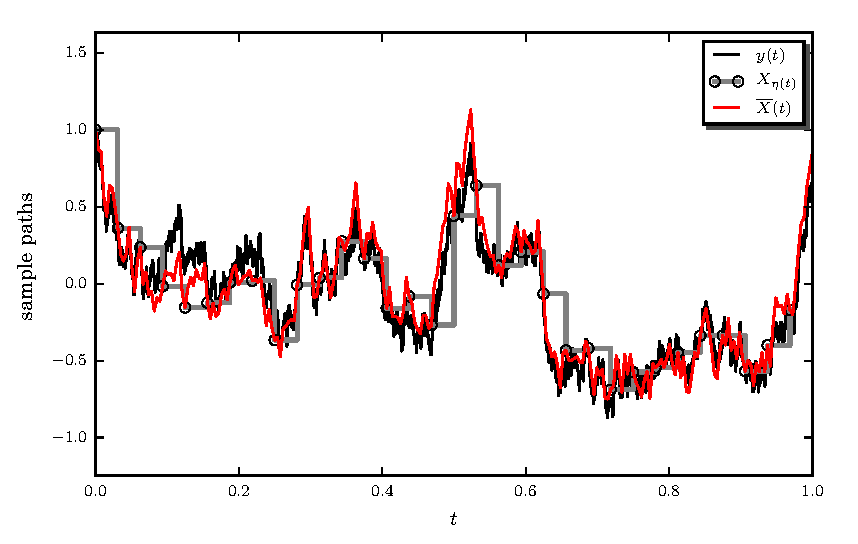
\includegraphics{papers/paperB/sections/ContinuousExtPy/ContinuousExtension.eps}
	\caption{
		The red line represents the continuous extension of the EM scheme. The continuous gray line is the 
		$Y_{\eta(t)}$ 
		process defined in \eqref{eqn:EulerMaruyama}.
	}
	\label{fig:ContinuousExtension}
\end{figure}
Using the continuous extension \eqref{eqn:EMContinuousExtension}
and the uniform mean square norm, the authors work with a stronger version of the ms-error%, which is given by 
$$
	\EX{\sup_{0\leq t \leq t}|y(t)-\overline{Y}(t)|^2}.
$$
%
Then, in  order to prove strong convergence of the EM method, the authors require the following assumptions.
\begin{assumption}\label{ass:HighamAssumption}
	For each $R>0$ there is a positive constant $C_R$, depending only on $R$, such that
	\begin{equation}\label{ass:LipschitzCondition}
		|f(x)-f(y)|^2 \vee |g(x)-g(y)|^2 \leq C_R|x-y|^2,
		\quad
		\forall x,y\in \R^d 
		\text{ with } |x|\vee |y|\leq R.
	\end{equation}
	And for some $p>2$, there is a constant $A$ such that
	\begin{equation}
		\EX{\sup_{0\leq t\leq T}|\overline{Y}(t)|^p}
		\vee
		\EX{\sup_{0\leq t\leq T}|y(t)|^p} \leq A.
	\end{equation}
\end{assumption}
In \cite{Higham2002b}, the authors prove that the \Cref{ass:HighamAssumption} is sufficient to ensure strong 
convergence for the EM scheme, namely 
\begin{thm}[
	{\cite[Thm 2.2]{Higham2002b}}
	]\label{thm:HighamMaoStuart}
	Under \Cref{ass:HighamAssumption}, the EM scheme \eqref{eqn:EulerMaruyama} with continuous extension
	\eqref{eqn:EMContinuousExtension}
	%\eqref{eqn:EMIntegralContinuousExtension} 
	satisfies
	\begin{equation}
		\lim_{h\to 0}
		\EX{\sup_{0\leq t\leq T}|\overline{Y}(t)-y(t)|^2}=0.
	\end{equation}
\end{thm}
	
	Applying this result, the authors prove the strong convergence of an implicit split-step variant of the EM, the
SSEM method. 
Their technique consist in proving each assertion of the following steps.
\begin{enumerate}[\bf{Step} 1:]
	\item
		\label{stp:EMCorrespondence}
		The SSEM for SDE \eqref{eqn:SDE1} is equivalent to the EM for the following conveniently SDE
		\begin{equation}\label{eqn:PerturbedHighamSDE}
			dy_h(t)= f_h(y_h(t))dt +g_h(y_h(t))dW(t).
		\end{equation}
	\item\label{stp:PerturbedSolution}
			The solution of the modified SDE \eqref{eqn:PerturbedHighamSDE} has bounded moments and it is 
			"close" to  $y$ the sense of the uniform mean square norm 
			$
				\EX{\sup_{0\leq t\leq T}|\cdot|^2}
			$.
	\item
	\label{stp:MethodBoundedMoments}
		Show that the SSEM method for the SDE \eqref{eqn:SDE1} has bounded moments.
	\item
		There is a continuous extension of the SSEM, $\overline{Z}(t)$, with bounded moments.
	\item
		Use the above steps and \Cref{thm:HighamMaoStuart} to conclude that
		\begin{equation}
			\lim_{h\to 0}
			\left\{
				\EX{\sup_{0\leq t\leq T}|y_h(t)-y(t)|^2}
			+
			\EX{\sup_{0\leq t\leq T}|\overline{Z}(t) -y_h(t)|^2}
			\right\}=0.
		\end{equation}
\end{enumerate}
In Chapter 4, we will use this technique.
% We will 
%use the same technique as these authors, that is, we will show that:
%\begin{inparaenum}[(a)]
%	\item
%		the underlying method corresponds to the EM for a perturbed SDE and
%	\item
%		all moments of the approximation are bounded.
%\end{inparaenum}
%
	\section{Strong Convergence of the Linear Steklov Method}
			Here, we state and prove the main result of this chapter, the strong convergence of the \SM method
 \crefrange{eqn:SSLSM1}{eqn:SSLSM2} for the solution of SDE \eqref{eqn:SDE1}.
The main idea of the proof consist in applying the technique discussed in \Cref{sec:HMS-Technique}.
We begin establishing the underlying convergence theorem.
\begin{thm} %[Strong Convergence of the \SM method]
%\begin{restatable}[Strong Convergence of the \SM]{theorem}{StrongConvergence}
	\label{thm:StrongConvergenceLSMethod}
	Let \Cref{ass:OSLC,ass:ajBound} hold, consider the \SM method \crefrange{eqn:SSLSM1}{eqn:SSLSM2} for the 
	SDE	\labelcref{eqn:SDE1}.
	Then there is a continuous-time extension $\overline{Y}(t)$ of the \SM solution $\{Y_k\}$ for which 
	$\overline{Y}(t_k)=Y_k$ and
	\begin{equation*}
	\lim_{h \to 0}
	\EX{
		\sup_{0\leq t \leq T}
		|\overline{Y}(t) - y(t)|^2	
	}=0.
	\end{equation*} 
\end{thm}
%\end{restatable}
%Before to apply the HMS technique we will prove
To proof this result, we initiate with the first step of the HMS technique, that is, we will show that the \SM method
for SDE \eqref{eqn:SDE1} is equivalent to the EM scheme applied to the conveniently modified SDE
	\begin{equation} \label{eqn:SDEMod}
		dy_h(t)= \varphi_{f_h}(y_h(t))dt +g_h(y_h(t))dW(t),
		\qquad y_h(0)=y_0,  \qquad t\in [0,T].
	\end{equation}
We formalize this as a Corollary of \Cref{lem:PhiFhProp}.
%======================================================================================================================
%                                                 STEP 1                                                              %
%======================================================================================================================

\begin{corollary}\label{col:SSSMeEMmod}
	Let \Cref{ass:OSLC,ass:ajBound} hold, then the \SM method for SDE \eqref{eqn:SDE1} is 
	equivalent to the EM scheme applied to the modified SDE \eqref{eqn:SDEMod}.
\end{corollary}
\begin{proof}
	Using the functions $\varphi_{f_h}(\cdot)$ and $g_h(\cdot)$ defined in \eqref{eqn:FunctionshDefinition} of 
	\Cref{lem:PhiFhProp}, we 
	can rewrite the \SM method \Crefrange{eqn:SSLSM1}{eqn:SSLSM2} as 
	$$
		Y_{k+1} = Y_k + h \varphi_{f_h}(Y_k) + g_h(Y_k)\Delta W_k,
	$$
	which is the EM approximation for the modified SDE \eqref{eqn:SDEMod}.
\end{proof}
%======================================================================================================================
%                                                 STEP 2                                                              %
%======================================================================================================================

	Now we proceed with the Step 2, that is,  we will prove that the solution  of the modified
SDE \eqref{eqn:SDEMod} has bounded moments and is close in uniform mean square norm to the solution of the SDE 
\eqref{eqn:SDE1}. In what follows we denote by $C$  a universal constant, that is, a positive constant
independent on h which value could change in occurrences.


\begin{lem}\label{lem:BoundAndConvergenceOfyh}
	Let \Cref{ass:OSLC,ass:ajBound,ass:HypThmSingularities} hold, then there is a universal 
	constant $C=C(p,T)>0$ and a sufficiently small
	step size $h$, such that for all $p>2$
	\begin{equation}\label{eqn:yh-MomentBounds}
		\m\left[
			\sup_{0\leq t \leq T}
				|y_h(t)|^p
		\right]
		\leq
			C
		\left( 
			1+\m |y_0|^p
		\right).
	\end{equation}
	Moreover
	\begin{equation}\label{eqn:yh-convergence}
	\lim_{h \to 0}
	\m\left[
	\sup_{0\leq t \leq T}
	|y(t)-y_h(t)|^2
	\right]=0.
	\end{equation}
\end{lem}
\begin{proof}
	By theorem \ref{thm:MaoCoercive} and inequality \eqref{eqn:h-MonotoneCondition}, 
	we have	 bound \eqref{eqn:yh-MomentBounds}.
	On the other hand, to prove \eqref{eqn:yh-convergence} we will use the properties of 
	$\varphi_{f_h}$ and the Higham's stopping time technique employed in \cite[Thm 2.2]{Higham2002b}. 
	Note that by relation \eqref{eqn:VarPhiEjc} of \Cref{lem:PhiFhProp} we have 
	\begin{align*}
		\varphi_{f_h}(x) 
			&= \Phi(h,a_j)(u) f^{(j)}(u) \1{E_j^c}(u) 
				+ f^{(j)}(u) \1{E_j}(u).
	\end{align*}
	
	By \Cref{ass:HypThmSingularities}  and since $f \in C^1(\R^d)$,   $\Phi(h,a_j)(\cdot)$ is bounded,
	hence, there is a positive constant $R_n$ which depends on $n$ such that 
	\begin{align*}	
		|\varphi_{f_h}^{(j)}(u) - f^{(j)}(u)|
		&\leq
			\1{E_j^c}(u)
			|f^{(j)}(u)|
			\left|
				\Phi(h,a_j)(u) - 1
			\right| \notag \\
		&\leq
			\1{E_j^c}(u)
			\left(
				L_{\Phi} + 1
			\right)
			|f(u)|	 \notag \\
		&\leq
		\1{E_j^c}(u) R_n(L_{\Phi}+1), \quad \forall u \in \R^d, \quad |u|\leq n,
	\end{align*}
	for each $j\in \{1,\dots, d\}$.
	
	
	Moreover, we know by the proof of \Cref{lem:PhiFhProp} that
	\begin{equation*}
	 \lim_{
	 	\substack{
		 	h\to 0 \\
		 	u\in E_j^c	
	 	}
	 }
	 \Phi(h,a_j)(u) = 1.	 	
	\end{equation*}
	Also, we note that for each $j \in \{1, \dots , d\}$
	\begin{equation*}
	\lim_{h \to 0} F_h^{(j)}(u)
		=
		\lim_{h \to 0}
			e^{ha_j(u)} u^{(j)} + 
		\lim_{h \to 0}
			\left(
				\frac{e^{ha_j(u)}-1}{a_j(u)}
				\1{E_j^c}(u)
				+h \1{E_j}(u)
			\right)
			b_j(u^{(j)}) 
		= u^{(j)},
	\end{equation*}
	hence
	$%\begin{equation*}
		\displaystyle
		\lim_{h\to 0} F_h(u)=u.
	$ %\end{equation*}
	Consequently, given $n>0$ there is  a function $K_n(\cdot):(0,\infty)\to (0,\infty)$, such that
	$K_n(h)\to 0$ when $h \to 0$ and
	\begin{equation}\label{eqn:PhihGhKRhBound}
		|\varphi_{f_h}(u)-f(u)|^2 \vee |g_h(u)-g(u)|^2
		\leq K_n(h) \qquad \forall u\in \R^d, \quad |u| \leq n.
	\end{equation}
	Now, using that both $f$, $g$ are $C^{1}$, there is  a constant $H_n>0$ such that
	\begin{equation}\label{eqn:f-gHRBound}
		|f(u)-f(v)|^2 \vee |g(u)-g(v)|^2
		\leq H_n |u-v|^2\qquad \forall u,v \in \R^d, |u|\vee |v| \leq n.
	\end{equation}
	
		On the other hand, by \Cref{lem:MomentBound} and inequality \eqref{eqn:yh-MomentBounds} we obtain
	\begin{equation*}
		\m\left[
			\sup_{0\leq t \leq T}
				|y(t)|^p
		\right]
		\vee
		\m\left[
			\sup_{0\leq t \leq T}
				|y_h(t)|^p
		\right]
		\leq
		K := C
		\left( 
			1+\m |y_0|^p
		\right).
	\end{equation*}
	Now, we define the stopping times
	\begin{equation}\label{eqn:StoppingTimes}
		\tau_n := 
			\inf\{
				t\geq 0: |y(t)|\geq n
			\},
		\qquad
		\rho_n := 
			\inf\{
				t\geq 0: |y_h(t)|\geq n
			\},
		\qquad
		\theta_n:=
			\tau_n \wedge \rho_n,
	\end{equation}
	and the difference function
	\begin{equation*}
		e_h(t):= y(t) - y_h(t).
	\end{equation*}
	From the Young's inequality \eqref{eqn:YoungsInequality}, we deduce that for any $\delta>0$ 
	\begin{align}
		\m\left[
			\sup_{0\leq t\leq T}
			|e_h(t)|^2
		\right]
		&=
			\m\left[
				\sup_{0\leq t\leq T}
				|e_h(t)|^2
				\1{\tau_n>T,\rho_n>T}
			\right]
			+
			\EX{
				\sup_{0\leq t\leq T}
				|e_h(t)|^2
				\1{\tau_n \leq T \text{ or } \rho_n \leq T}
			}\notag\\
		&\leq
			\EX{
				\sup_{0\leq t\leq T}
				|e_h(t\wedge \theta_n)|^2
				\1{\theta_n \geq T}
			}
			+\frac{2\delta}{p}
			\EX{
				\sup_{0\leq t\leq T}
				|e_h(t)|^p 
			}\notag \\
		&+
			\frac{1-2/p}{\delta^{2/(p-2)}}
			\Prob{\tau_n \leq T \text{ or } \rho_n \leq T}.
	\label{eqn:AfterYoungIneq}
	\end{align}
	We proceed to bound each term on the right-hand side of inequality \eqref{eqn:AfterYoungIneq}.
	By \Cref{lem:MomentBound}, $y(t)$ has bounded moments, hence 
	there is a positive constant $A$ such that
	\begin{equation}\label{eqn:BoundProbTauR}
		\Prob{\tau_n\leq T}
		=
			\EX{\1{\tau_n<T}\frac{|y(\tau_n)|^p}{n^p}}
		\leq
			\frac{1}{n^p}\EX{\sup_{0\leq t\leq T}|y(t)|^p} \leq \frac{A}{n^p},
			\qquad \text{for } p\geq 2.
	\end{equation}
	The same conclusion can be drawn for $\rho_n$, then
	\begin{equation} \label{eqn:BoundProbTauRorRhoR}
		\Prob{\tau_n \leq T \text{ or } \rho_n \leq T}
		\leq
			\Prob{\tau_n\leq T}+\Prob{\rho_n\leq T}
		\leq
		\frac{2A}{n^p}.
	\end{equation}
	Now, using the inequality \eqref{eqn:SingleHolder} and \Cref{lem:MomentBound} we have
	\begin{equation} \label{eqn:ehMomentBound}
		\EX{
			\sup_{0\leq t \leq T}
			|e_h(t)|^p
		}
		\leq
		2^{p-1}
		\EX{
			\sup_{0 \leq t \leq T}
			\left(
			|y(t)|^p + |y_h(t)|^p
			\right)
		}
		\leq 2^pA.
	\end{equation}
%
	So, combining the bound \eqref{eqn:BoundProbTauRorRhoR} with \eqref{eqn:ehMomentBound}
	in inequality \eqref{eqn:AfterYoungIneq} we obtain
	\begin{align}
		\EX{
			\sup_{0\leq t \leq T}
			|e_h(t)|^2
		}
		&\leq
			\EX{
				\sup_{0\leq t\leq T}
				|e_h(t\wedge \theta_n)|^2
				\1{\theta_n \geq T}
			}
	%\notag \\
			+\frac{2^{p+1}\delta A}{p}
			+\frac{2(p-2)A}{p\delta^{2/(p-2)}n^p}. \label{eqn:TermToBound}
	\end{align}
	Next, we show that the first term of \eqref{eqn:TermToBound} is bounded. Adding conveniently terms yields
	\begin{align*}
		e_h(t\wedge\theta_n) 
			&=
			\int_{0}^{t\wedge\theta_n}
			\left[
				f(y(s)) - f(y_h(s))+f(y_h(s))
				-\varphi_{f_h}(y_h(s))
			\right]ds \notag \\
			&+
			\int_{0}^{t\wedge\theta_n}
			\left[
				g(y(s)) - g(y_h(s))+g(y_h(s))
				-g_h(y_h(s))
			\right]dW(s).
	\end{align*}
	Using the bounds \eqref{eqn:PhihGhKRhBound} and \eqref{eqn:f-gHRBound}, the Cauchy-Schwarz, and
	Doob martingale inequalities, we get
	\begin{align*}
		\EX{\sup_{0\leq t \leq \tau}|e_h(t\wedge\theta_n)|^2}
		&\leq 
		4H_n(T+4)
		\int_{0}^{\tau}
			\EX{\sup_{0\leq t \leq \tau}|e_h(t\wedge\theta_n)|^2} ds 
		+
		4T(T+4)K_n(h).\notag
	\end{align*}
	The Gronwall inequality now yields
	\begin{align*}
		\EX{\sup_{0\leq t \leq T}|e_h(t\wedge\theta_R)|^2}
		&\leq
			4T(T+4)K_n(h)\exp(4H_n(T+4)T). %\notag \\
	%+
	%\frac{2^{p+1}\delta A}{p}
	%+
	%\frac{(p-2)2A}{p\delta^{2/(p-2)}R^p}.
	\end{align*}
	Hence, given $\epsilon>0$ for any $\delta>0$ such that
	$
		2^{p+1}\delta A/p< \epsilon/3,
	$
		we can take $n>0$ verifying
	$
		(p-2)2A/(p\delta^{2/(p-2)}n^p)<\epsilon/3.
	$
	Moreover, we can take $h$ sufficiently small such that
	$
		4T(T+4)K_n(h)\exp(4H_n(T+4)T) < \epsilon/3. 
	$
	It follows immediately that
	$$
		\EX{\sup_{0\leq t \leq T}|e_h(t)|^2}
		<
			\epsilon/3
			+\epsilon/3
			+\epsilon/3
		=\epsilon,
	$$ which is the desired conclusion.
\end{proof}
%======================================================================================================================
%                                                 STEP 3                                                              %
%======================================================================================================================

	Next, we proceed with Step 3, in which we establish that \SM method has bounded moments.
\begin{lem}\label{lem:SSSMMomentBounds}
	Let \Cref{ass:OSLC,ass:ajBound,ass:HypThmSingularities} hold. Then for each $p\geq 2$ there is 
	a universal positive constant  $C=C(p,T)$ 
	such that the explicit \SM method
	\begin{equation*}
		\m\left[
		\sup_{kh \in [0,T]}
		|Y_k|^{2p}
		\right]\leq C.
	\end{equation*}
\end{lem}
\begin{proof}
Denoting by  $A^{(i)}_k:= A^{(i)} (h,Y_k)$ for $i=1,2$ and $b_k:=b(Y_k)$, we use
a split formulation of the \SM scheme \crefrange{eqn:SSLSM1}{eqn:SSLSM2} as follows:
\begin{eqnarray*}
	Y_{k}^{{\star}^{(j)}} &=& A^{(1)}_k Y_k + A^{(2)}_k b_k, \label{split1}\\
	Y_{k+1}^{(j)}&=& Y_k^{{\star}^{(j)}} + g^{(j)}(Y_k^{\star})\, \Delta W_k 
	\label{split2},
\end{eqnarray*}
from the first step of this split scheme, using (A-3) and 
the Cauchy-Schwartz inequality, we get
\begin{eqnarray}
|Y_k^{\star}|^{2}
&\leq&
|A^{(1)}_k |^2 |Y_k|^2  
+ 2 \innerprod{A^{(1)}_k Y_k}{A^{(2)}_k Y_k 
	b_k}
+|A^{(2)}_k|^2 |b_k|^2\nonumber\\
&\leq&
|A^{(1)}_k|^2 |Y_k|^2  
+ 2 \sqrt{L_b} d|A^{(1)}_k||A^{(2)}_k||Y_k|(1+|Y_k|)
+L_b|A^{(2)}_k|^2 (1+|(Y_k)|^2).\label{leqn:Yn2Bound} 
\end{eqnarray}
From (A-2), we can deduce that
\begin{dmath}[label=eqn:A1Bound]
	|A^{(1)}_k|^2 
	=
	\left|
	\diag
	\left(
	e^{ha_1(Y_k)}, \dots, e^{ha_d(Y_k)} 
	\right)
	\right|^2
	\leq L_{A^{(1)}},		
\end{dmath}
where $L_{A^{(1)}}=d\, e^{ 2 T L_a}$ and also by \eqref{eqn:PhiBound}, we can derive that
\begin{align}
	|A^{(2)}(h,Y_k)|^2 
	&=
	\left|
	h 
	\diag
	\left(
	\1{E_1}(Y_k)
	+\1{E_1^c}(Y_k)\Phi_1(Y_k), 
	\dots,
	\1{E_d}(Y_k)
	+\1{E_d^c}(Y_k) \Phi_d(Y_k)
	\right)
	\right|^2 \notag \\
	%
	&\leq
	\sum_{j=1}^{d}
	\left(
	\1{E_j^c}
	|h\Phi_j(Y_k)|^2
	+ h^2
	\right)
	\leq
	2 e^{2 L_a  T}
	\sum_{j=1}^d
	\frac{1}{a_j^*} + d T^2\leq L_{A^{(2)}}.
	\label{eqn:A2Bound}
\end{align}
Substituting \eqref{eqn:A1Bound} and \eqref{eqn:A2Bound}  on  inequality \eqref{leqn:Yn2Bound} yields
\begin{eqnarray*}\label{eqn:YkStarBound}
	|Y_k^{\star}|^2
	&\leq&	L_{A^{(1)}} |Y_k|^2
	+ 2 d \sqrt{L_{A^{(1)}} L_{A^{(2)}} L_b }\,|Y_k|(1+|Y_k|)
	+L_{A^{(2)}} L_b (1+|Y_k|^2)		
	\leq C(1+|Y_k|^2),
\end{eqnarray*}
where $C\geq L_{A^{(1)}}+ 2 d \sqrt{L_{A^{(1)}} L_{A^{(2)}} L_b} + 
L_{A^{(2)}} L_b$. Applying  bound \eqref{eqn:YkStarBound} 
in the  second step of the split scheme, we get
\begin{equation*}
	|Y_{k+1}|^2
	\leq
	C \left(
	|Y_k|^2 + 1
	\right)
	+ 2\innerprod{Y^{\star}_k}{g(Y^{\star}_k) \Delta W_k}
	+ \left|g(Y^{\star}_k) \Delta W_k \right|^2.
\end{equation*}
Now, we choose two integers $N,M$ such that $Nh\leq Mh \leq T$. So, adding 
backwards we obtain
\begin{equation*}
	|Y_N|^2
	\leq
	S_N\left(
	\sum_{j=0}^{N-1}
	(1+|Y_j|^2)
	+
	2\sum_{j=0}^{N-1}
	\innerprod{Y_j^{\star}}{g(Y_j^{\star}) \Delta W_j}
	+
	\sum_{j=0}^{N-1}
	\left|
	g(Y_j^{\star}) \Delta W_j
	\right|^2
	\right),
\end{equation*}
where	$S_N:=	\sum_{j=0}^{N-1}C^{N-j}$. Raising both sides to the 
power $p$,  we get
\begin{align}\label{eqn:RelationToBound}
	|Y_N|^{2p}	
	&\leq
	6^{p} S_N^p
	\left(
	N^{p-1}
	\sum_{j=0}^{N-1}
	(1+|Y_j|^{2p})	
	+
	\left|
	\sum_{j=0}^{N-1}
	\innerprod{Y_j^{\star}}{g(Y_j^{\star}) \Delta W_j}
	\right|^p
	+
	N^{p-1}
	\sum_{j=0}^{N-1}
	\left|
	g(Y_j^{\star}) \Delta W_j
	\right|^{2 p}				
	\right).
\end{align}
Now we will show that the second and third terms of inequality \eqref{eqn:RelationToBound} are bounded.
We denote by $C=C(p,T)$ a generic positive constant which does not depend on  the step size $h$ and whose
value may change between occurrences.	Next, applying the Bunkholder-Davis-Gundy
inequality  \cite{Mao2007}, we have
\begin{eqnarray}\label{eqn:BoundSecondTerm}
\m
\left[
\sup_{0\leq N \leq M}
\left|
%\exp(2hpNL)
\sum_{j=0}^{N-1}
\innerprod{Y_j^{\star}}{g(Y_j^{\star})\Delta W_j}
\right|^{p}
\right]
&\leq&
C\m
\left[
\sum_{j=0}^{N-1}
|Y_j^{\star}|^2
|g(Y_j^{\star})|^2
h
\right]^{p/2}
\notag\\
&\leq&
C h^{p/2}M^{p/2-1}
\m
\sum_{j=0}^{M-1}
|Y_j^{\star}|^p (\alpha +\beta |Y_j^{\star}|^2)^{p/2}
\notag\\
&\leq&
2^{p/2-1}C T^{p/2-1} h  
\m
\sum_{j=0}^{M-1}
(\alpha^{p/2}|Y_j^{\star}|^p +\beta^{p/2} |Y_j^{\star}|^{2p})
\notag\\
&\leq&
C h
\m
\sum_{j=0}^{M-1}
(1+2|Y_j^{\star}|^p + |Y_j^{\star}|^{2p})
\notag\\
&\leq&
C 
+ 
C h 
\sum_{j=0}^{M-1}
\m|Y_j|^{2p},				
\end{eqnarray}
Now, using the Cauchy-Schwartz inequality, the monotone condition 
\eqref{eqn:MonotoneCondition} and bound \eqref{eqn:YkStarBound}, we obtain
\begin{eqnarray}
\m\left[
\sup_{0\leq N \leq M}
\sum_{j=0}^{N-1}
\left|
g(Y_j^{\star})\Delta W_j
\right|^{2p}	
\right]
&\leq&	
\sum_{j=0}^{M-1}
\m
\left|
g(Y_j^{\star})
\right|^{2p}
\m
\left|
\Delta W_j
\right|^{2p}
\notag \\
&\leq&
C h^p
\sum_{j=0}^{M-1}
\m
\left[
\alpha +\beta|Y^{\star}_j|^2
\right]^p
\notag\\
%
&\leq&
Ch^p
\sum_{j=0}^{M-1}
\m
\left[
\alpha ^p +\beta^p |Y^{\star}_j|^{2p}
\right]
\notag\\
&\leq&
Ch^{p-1}
+
Ch^p \sum_{j=0}^{M-1}
\m|Y_j|^{2p} \label{eqn:BoundThirdTerm}.
\end{eqnarray}
Thus, combining bounds \eqref{eqn:BoundSecondTerm} and \eqref{eqn:BoundThirdTerm} with inequality 
\eqref{eqn:RelationToBound}, we can assert that
\begin{align}
	\EX{
		\sup_{0\leq N \leq M}
		|Y_N|^{2p} 
	}
	% 		\leq
	% 			C(M,T) + C(M,T)(1+h)
	% 			\sum_{j=0}^{M-1}
	% 				\m|Y_j|^{2p}
	\leq	
	C +C(1+h) 
	\sum_{j=0}^{M-1}
	\EX{
		\sup_{0\leq N \leq j}
		|Y_N|^{2p}
	}	
	.
\end{align}
Finally, using the discrete-type Gronwall inequality \cite{Mao2007}, we conclude that
\begin{align*}
	\EX{
		\sup_{0\leq N \leq M}
		|Y_N|^{2p} 
	}	
	&\leq
	C e^{C(1+h)M} 
	\leq 
	C e^{C(1+T)}<C,
\end{align*}
since the constant C does not depend on $h$, the proof is complete.
\end{proof}

%======================================================================================================================
%                                                 STEP 4                                                              %
%======================================================================================================================
	
	Since the \SM scheme has bounded moments, we now proceed whit Step 4, that is,  we will obtain a convenient 
continuous extension of the \SM method with bounded moments. 
Let $\{Y_k\}$ denote the \SM solution of SDE \eqref{eqn:SDE1}.
By \Cref{col:SSSMeEMmod}, we conveniently made a continuous extension for the \SM approximation, from the 
time continuous extension of the EM \eqref{eqn:EMContinuousExtension}.
Moreover, we prove that the  moments of this extension remains bounded.
\begin{corollary}\label{col:ContinuousExtBoundedMoments}
	Let \Cref{ass:OSLC,ass:ajBound,ass:HypThmSingularities} holds and suppose  $0<h<1$ and $p\geq 
	2$. Then there is a continuous extension $\overline{Y}(t)$ of $\{Y_k\}$  and a universal constant $C=C(T,p)$ such 
	that
	\begin{equation*}
		\EX{\sup_{0\leq t \leq T} |\overline{Y}(t)|^{2p} }
		\leq C.
	\end{equation*}
\end{corollary}
	\begin{proof}
		We take $t=s+t_k$ in $ [0,T]$, $\Delta W_k(s):= W(t_k+s)- W(t_k)$ and $0\leq s <h$.
		Then we define 
		\begin{equation}\label{eqn:SSLSContinuousExtension}
			\overline{Y}(t_k+s):= Y_k + s \varphi_{f_h}(Y_k) + g_h(Y_k)\Delta W_k(s),
		\end{equation}
		as a continuous extension of the \SM scheme. We proceed to show that $\overline{Y}(t)$ has bounded moments.
		By \Cref{lem:PhiFhProp}, we have $Y_k^{\star}= Y_k + h \varphi_{f_h}(Y_k)$. 
		Then for $\gamma = s/h$, it follows that
		\begin{align*}
			Y_k + s \varphi_{f_h}(Y_k)
			&= 
			\gamma (Y_k + h \varphi_{f_h}(Y_k)) +(1-\gamma)Y_k\\
			&=
			\gamma Y_k^{\star} + (1-\gamma)Y_k.
		\end{align*}
		Hence, we can rewrite the continuous extension \eqref{eqn:SSLSContinuousExtension} as
		\begin{align}
			\overline{Y}(t) &=
			\gamma Y^{\star}_k + (1-\gamma) Y_k +g_h(Y_k) \Delta W_k(s). %\label{eqn:SSLSMConExt}
			\notag
		%t&=t_k+s,  \qquad  \gamma = s/h\qquad s\in {[0,h)]}.\notag
		\end{align}
		%
		Combining this relation with  the inequalities \eqref{eqn:YkStarBound} and \eqref{eqn:SingleHolder}, we arrive 
		at
		\begin{align}
			|\overline{Y}(t_k+s) |^2 
			&\leq
				3\left[
					\gamma C
					+
					\left(
						\gamma C +1 - \gamma
					\right)
					|Y_k|^2
					+
					|g_h(Y_k)\Delta W_k(s)|^2
			\right] \notag\\
		&\leq
			C
			+
			C
			\left(
				|Y_k|^2 + |g_h(Y_k)\Delta W_k(s)|^2
			\right).
		\notag
		\end{align}
	Thus, 
	\begin{align}
		\sup_{0\leq t\leq T} |\overline{Y}(t)|^{2p}
		&\leq
			\sup_{0\leq kh\leq T}
			\left[
				\sup_{0\leq s\leq h}
					|\overline{Y}(t_k+s)|^{2p} 
			\right] 
		\notag\\
		&\leq
			\sup_{0\leq kh\leq T} 
			\left[
				\sup_{0\leq s\leq h}
					C 
					\left(
						1 + |Y_k|^{2p} + |g_h(Y_k)\Delta W_k(s)|^{2p}
					\right)
			\right],
		\label{eqn:BeforeDoob}
	\end{align}
	for $t\in [0,T]$.
	%
	Now taking a non negative integer $0 \leq k \leq N$ such that $0\leq Nh \leq T$. From the bond 
	\eqref{eqn:BeforeDoob}, we get
	\begin{align}
		\sup_{0\leq t\leq T} |\overline{Y}(t)|^{2p}
		&\leq 
			C
			\left(
				1
				+
				\sup_{0\leq kh\leq T} 
					|Y_k|^{2p}
					+
					\sup_{0\leq s\leq h}
						\sum_{j=0}^N
							|g_h(Y_j)\Delta W_j(s)|^{2p}
			\right) \label{eqn:SumDiffusion}.
	\end{align}
	So, using the Doob's Martingale inequality \eqref{eqn:DoobMartingaleInequality},
	\Cref{lem:SSSMMomentBounds} and that $g_h$ is a locally 
	Lipschitz function, we can bound each term of the inequality \eqref{eqn:SumDiffusion},  as follows
	\begin{align}
		\EX{
			\sup_{0 \leq s \leq h} |g(Y_j) \Delta W_j(s)|^{2p}
		}
		&\leq
			\left(
				\frac{2p}{2p-1}
			\right)^{2p}
			\m|g_h(Y_j)\Delta W_j(h)|^{2p}
			\notag
			\\
		&\leq
			C \m |g_h(Y_j)|^{2p} \m |\Delta W_j(h)|^{2p} \notag\\
		&\leq
			C h^p
			\left(
				1 + \m|Y_j|^{2p}
			\right) \notag \\
		& \leq C h, \label{eqn:BeforeConclusion}
	\end{align}
	for each $j \in \{0,\dots, N\}$.
	Since $Nh\leq T$, combining the bounds \eqref{eqn:SumDiffusion} and \eqref{eqn:BeforeConclusion} we 
	get the desired conclusion.
	\end{proof}
%======================================================================================================================
%                                                 STEP 5                                                              %
%======================================================================================================================

	Once we have carried out all the previous steps, we can prove the \Cref{thm:StrongConvergenceLSMethod} by Step 5.%
%We are now in a position to execute the \textbf{Step 5}.
\begin{proof}[Proof of \Cref{thm:StrongConvergenceLSMethod}]
	First,  note that by inequality \eqref{eqn:SingleHolder}, we have
	\begin{align}\label{eqn:AfterTriangle}
		\EX{\sup_{0\leq t \leq T}|\overline{Y}(t) - y(t)|^2}
		&\leq
		2\EX{
			\sup_{0\leq t \leq T}
			|\overline{Y}(t) - y_h(t)|^2
		}
		+
		2\EX{
			\sup_{0\leq t \leq T}
			|y_h(t) - y(t)|^2
		}.
	\end{align}
	Using \Cref{lem:BoundAndConvergenceOfyh}, which was established in the Step 2, yields
	\begin{equation}\label{eqn:SeconTermZeroLim}
		\lim_{h\to 0}
		\EX{
			\sup_{0\leq t \leq T}
			|y_h(t) - y(t)|^2
		} = 0.
	\end{equation}
	
		It remains to prove that the first term of the right hand side in inequality \eqref{eqn:AfterTriangle} 
		decreases to zero
	when $h$ tends to zero. Recalling that:
	\begin{enumerate}[i)]
	%\begin{inparaenum}[\itshape i\upshape)]
		\item 
			By \Cref{lem:BoundAndConvergenceOfyh}, the solution of the modified SDE \eqref{eqn:SDEMod}, $y_h$, has
			$p$-bounded moments ($p\geq 2$).
		\item
			By \Cref{col:ContinuousExtBoundedMoments}, the \SM continuous extension for the SDE \eqref{eqn:SDE1},
			$\overline{Y}(t)$, has bounded moments and it is equivalent to the EM extension for the modified SDE 
			\eqref{eqn:SDEMod}.
		%\end{inparaenum}
	\end{enumerate}
	Hence, we can apply 
	%\cite[Thm. 2.2]{Higham2002b} 
	\Cref{thm:HighamMaoStuart} to conclude that
	\begin{equation}\label{eqn:FirstTermZeroLim}
		\lim_{h\to 0}
		\EX{
			\sup_{0\leq t \leq T}
			|\overline{Y}(t) - y_h(t)|^2
		} = 0.
	\end{equation}
	Finally, combining the limits \eqref{eqn:SeconTermZeroLim} and \eqref{eqn:FirstTermZeroLim} with 
	inequality \eqref{eqn:AfterTriangle} gives
	\begin{align*}
		\lim_{h \to 0}
		\EX{
			\sup_{0\leq t \leq T}
			|\overline{Y}(t) - y(t)|^2
		}
		&\leq	
		2\lim_{h\to 0}
		\EX{
			\sup_{0\leq t \leq T}
			|\overline{Y}(t) - y_h(t)|^2
		}
		\\
		&
		+
		2\lim_{h\to 0}
		\EX{
			\sup_{0\leq t \leq T}
			|y_h(t) - y(t)|^2
		} = 0,
	\end{align*}
	which proves the theorem. 
\end{proof}
%
	\section{Convergence Rate}
			In this section we show that the explicit Linear Steklov method 
\cref{eqn:SSLSM1,eqn:SSLSM2} converges  with a standard order of one-half. For that,
we use a similar procedure  as in  \cite{Higham2002b}. In addition 
to \Cref{ass:OSLC,ass:ajBound,ass:HypThmSingularities} we also require the following.
 
 \begin{hypothesis}\label[hypothesis]{ass:PolynomialGrowth}
 	There exist constants $L_f, D\in \R$ and $q \in \Z^+$ such that $\forall u,v \in \R^d$
 	\begin{align}
 	\innerprod{u-v}{f(u)-f(v)}
 	&\leq L_f|u-v|^2, \\
 	|f(u) - f(v)|^2 
 	&\leq 
 	D(1 + |u|^q +|v|^q) |u-v|^2.
 	\end{align}
 \end{hypothesis}
 
 \begin{hypothesis}\label[hypothesis]{ass:MomentBounds}
 	The SDE \eqref{eqn:SDE1}  the EM solution and its continuous extension satisfy
 	\begin{equation}
 	\EX{
 		\sup_{0\leq t\leq T}
 		|y(t)|^p	
 	}, \quad
 	\EX{
 		\sup_{0\leq t\leq T}
 		|Y(t)|^p	
 	}, \quad
 	\EX{
 		\sup_{0\leq t\leq T}
 		|\overline{Y}(t)|^p	
 	} < \infty, \qquad \forall p\geq 1.
 	\end{equation}
 \end{hypothesis}

 \begin{thm}\label{thm:EulerConvergenceRateHMS}[{\citet[Thm 4.4]{Higham2002b}}]
 	Under \Crefrange{ass:ajBound}{ass:PolynomialGrowth} the EM solution with continuous extension $\overline{X}$
 	satisfies
 	\begin{equation}
 	\EX{
 		\sup_{0\leq t \leq T}
 		|\overline{Y}(t)- y(t)|^2
 	} = \mathcal{O}(h^2).
 	\end{equation}
 \end{thm}
  
\begin{lem}
	Under \Cref{ass:PolynomialGrowth,ass:MomentBounds} and sufficiently small $h$, there exist
	constants $D'\in \R$ and $q'\in \Z$ such that for all $u,v\in \R^d$
	\begin{align}
		|
			\varphi_{f_h}(u)
			-\varphi_{f_h}(v)
		|^2 
		&\leq
			D'
			\left(
				1 +|u|^{q'} +|v|^{q'}
			\right)
			|u-v|^2, \\
		%
		|
			 f(u) -\varphi_{f_h}(u)
		|^2 
		&\leq
			D'
			\left(
				1 +|u|^{q'} 
				\right)
			h^2, \\
		%
		|
			g(u) -g_h(u)
		|^2 				 
		&\leq
			D'
			\left(
				1 +|u|^{q'} 
			\right)
			h^2 . \label{eqn:ghPolyGrowth}
	\end{align}
\end{lem}

\begin{pf}
	From inequality \eqref{eqn:PhifhFbound}, we have
	\begin{equation*}
		|\varphi_{f_h}(u) - \varphi_{f_h}(v)|^2
		\leq
			(2 + L_{\Phi}) |f(u) - f(v)|^2 
			\leq
				(2 + L_{\Phi}) D (1 + |u|^q +|v|^q). 
	\end{equation*}
	Moreover, if $u \in E_j$ then $\varphi_{f_h}(u) = f^{(j)}(u)$. On the other hand,  if $u\in E_j^c$ then
	$$
		|f(u) - \varphi_{f_h}(u)|^2
		=
		\sum_{j=1}^d
			|1-\Phi(h,a_j)(u)|^2 |f^{(j)}(u)|^2,	
	$$
	 By the L'H\^{o}pital 
	theorem, we get
	\begin{align*}
		\lim_{h \to 0} |1-\Phi(h,a_j)(u)| 
			&= \left|
				1-\lim_{h\to 0} \frac{e^{h a_j(u)}-1}{h a_j(u)}
			\right|			
			\leq 
				\left|
					1-\lim_{h\to 0} e^{h L_a}
				\right|=0.			
	\end{align*}
	Thus, there is a sufficiently small $h>0$  such that
	$|1-\Phi_j(u)|<C h$ for all $u\in E_j^c$ and
	$$
		|f(u) - \varphi_{f_h}(u)|^2
		\leq
		Ch^2 |f(u)|^2
		\leq D'(1+|u|^q)h^2,	
	$$
	as we require. Given that $g_h(u)=g(F_h(u))$ from 
	theorem \ref{lem:PhiFhProp} we get
	\begin{equation*}
		|g(u) - g_h(u)|^2 
		\leq
			L_g |u - u +h \varphi{f_h}(u)|^2 
		\leq 
			2(1+L_{\Phi})h^2 |f(u)|^2
		\leq
			2(1+L_{\Phi}) D(1+|u|^q) h^2. 
	\end{equation*}
	\qed
\end{pf}
%
\begin{lem}\label{lem:yhyOh}
	Assume \Cref{ass:PolynomialGrowth,ass:MomentBounds} hold then the solution $y_h(t)$ of 
	the modified SDE \eqref{eqn:PerturbedHighamSDE}
	satisfies
	\begin{equation}
		\EX{
			\sup_{0\leq t \leq T}
			|y_h(t) - y(t)|^2	
		} = \mathcal{O}(h^2).
	\end{equation}	
\end{lem}
\begin{pf}
	We define $e(t):= y(t)-y_h(t)$ where
	\begin{eqnarray*}
		y(t) &=& y_0 + \int_{0}^t f(y(s))ds + \int_{0}^t g(y(s))dW(s),  \nonumber\\
		y_h(t) &=& y_0 + \int_{0}^t \varphi_{f_h}(y_h(s))ds + \int_{0}^t 
		g_h(y_h(s))dW(s).\nonumber
	\end{eqnarray*}
	Using It\^{o}'s formula over the function $V(t,x,y) = |x-y|^2$ for all  $x,y\in \R^d$, we obtain 
$$
		d e(t) = 
		\left(
			f(y(t)) - \varphi_{f_h}(y(t)) dt
		\right)
		+
		\left(
			g(y(t)) - g_h(y_h(t))
		\right) dW(t),
	$$
	Thus,
	\begin{align} \label{eqn:IntErrToBound}
		|e(t)|^2 
		&=
			2 \underbrace{\int_{0}^t
				\innerprod{e(s)}{f(y(s))-\varphi_{f_h}(y_h(s))} ds }_{:=I_1}
			+
			\underbrace{\int_{0}^t
				|g(y(s)) - g_h(y_h(s))|^2 ds }_{:=I_2}\notag\\
		&+
			2 \underbrace{\int_{0}^t
				\innerprod{e(s)}{\left[ g(y(s))-g_h(y_h(s)) \right] dW(s)}}_{:=I_3}.	\end{align}
	Now we proceed to bound each integral of inequality \eqref{eqn:IntErrToBound}. 
	By \Cref{ass:PolynomialGrowth} and the Young inequality, we get
	\begin{align*}
		I_1(t) 
		&\leq
			2\int_0^t
				\innerprod{y(s) - y_h(s)}{f(y(s))-f(y_h(s))} ds
			+
			 \int_0^t
				 \innerprod{y(s) - y_h(s)}{f(y_h(s))-\varphi_{f}(y_h(s))} ds \notag\\
%	
		&\leq
			3\int_0^t
				|y(s) - y_h(s)|^2ds
			+ D' h^2 
			\int_0^t
				1 + |y_h(s)|^{q'} ds.
	\end{align*}
	Since $y_h(t)$  the has bonded moments, there exists a universal constant $L$ which does not depends on $h$ 
	such that
	\begin{equation}\label{eqn:I1Bound} 
		 \EX{
			 I_1(s)	
		 }
		 \leq
			 L\int_{0}^t
				\m{|e(s)|^2} ds
		+ L h^2.
	 \end{equation}
	Using  \Cref{ass:OSLC,ass:PolynomialGrowth} it is followed
	\begin{align*}
		I_2(t) 
		&\leq
			2 L_g 
			\int_{0}^t
				|y(s) - y_h(s)|^2 ds
			+
			2D'h^2
			\int_0^t
				1 + |y_h(s)|^q ds, 	 
	\end{align*}
	thus
	\begin{equation} \label{t5}
		\EX{
			I_2(s)	
		}
		\leq
		L\int_{0}^t
		\m{|e(s)|^2} ds
		+ L h^2.
	\end{equation}
	Note that $\EX{ I_3(t)} \leq \EX{ 
				\sup_{0\leq s \leq t}
				|I_3(s)|
			}$.
	From the Burkholder-Davis-Gaundy inequality, \Cref{ass:OSLC,ass:PolynomialGrowth} and 
	as $y_h(t)$ has bounded moments, we obtain
	\begin{align}
		\EX{ 
			\sup_{0\leq s \leq t}
			|I_3(s)|
		}
		%
		&\leq
		2^4 
		\EX{
			\sup_{0 \leq s \leq t}
			|e(s)|^2
			\int_{0}^t
				|g(y(s))-g_h(y(s))|^2 ds
		}^{1/2} \notag \\
		&\leq
		2^4 
		\EX{
			\frac{1}{2 \cdot 2^9}
			\left(
				\sup_{0\leq s \leq t}
				|e(s)|^2
			\right)			
			+
			\frac{2^9}{2}
			\left(
				\int_{0}^t
					|g(y(s)) - g_h(y_h(s))|^2 ds
			\right)^2
		}
		\notag \\
		&\leq
			2 L_g
			\EX{
				\int_{0}^t
					|y(s) - y_h(s)|^2 ds		
				} 
			+D'Th^2 
			+
			D'Th^2
			\int_{0}^t
				\m{|y_h(s)|^{q'}} ds 	
		\notag \\
		&\leq
			L
			\int_{0}^t
				\m |e(s)|^2 ds
			+L h^2. \label{eqn:I3Bound}
	\end{align}
	Substituting inequalities \eqref{eqn:I1Bound}, \eqref{t5} and \eqref{eqn:I3Bound} 
	on equation \eqref{eqn:IntErrToBound}, we deduce that
	\begin{equation*}
		\EX{
			\sup_{0\leq s \leq t}	
			|e(t)|^2
		}
		\leq
			L \int_0^t
				\m |e(s)|^2 ds
			+
			L h^2 
		\leq		
			L \int_{0}^t
				\EX{
					\sup_{0\leq r \leq s}
					|e(s)|^2	
				}ds
			+Lh^2.		
	\end{equation*}
	By the Gronwall inequality, we conclude that
	\begin{equation*}
		\EX{
			\sup_{0 \leq t \leq T} 	
			|e(t)|^2
		}
		\leq
			L  \exp(LT) h^2 \leq C h^2. 
	\end{equation*} 	\qed
		
\end{pf}

	We  can now obtain the convergence rate of the explicit Linear Steklov method.

\begin{thm}
	Under \Crefrange{ass:OSLC}{ass:PolynomialGrowth} and consider the explicit \SM method 
	\eqref{eqn:SolutionFunctions} for the SDE \eqref{eqn:SDE1}.
	Then there exists a continuous-time extension $\overline{Y}(t)$ of the 
	LS numerical approximation for which
	\begin{equation} \label{orden}
		\EX{
			\sup_{0 \leq t \leq T}
			|\overline{Y}(t) - y(t)|^2	
		} = \mathcal{O}(h).	
	\end{equation}
\end{thm}
\begin{pf} Using bound  \eqref{eqn:AfterTriangle} then by  lemma \ref{lem:yhyOh} and since
 the LS continuous-time extension \eqref{eqn:SSLSContinuousExtension} is equivalent to the EM continuous-time extension 
 \eqref{eqn:EMContinuousExtension}, 
 we can use \Cref{thm:EulerConvergenceRateHMS} and conclude that the \SM has order one-half. \qed
\end{pf}

	\section{Numerical Experiments}
		Here we analyze the behavior of the explicit Linear Steklov method (\SM) for scalar and vector SDEs. 
The tests confirm the convergence order 1/2 for stochastic differential systems with locally Lipschitz drift 
and suggest that the \SM scheme reproduces almost surely stability (a.s.). We validate the efficiency of the new 
method  by comparing with other actual methods like the Euler-Maruyama, Backward-Euler-Maruyama (BEM) \cite{Mao2013} 
and Tamed-Euler-Maruyama (TEM) \cite{Hutzenthaler2012a}. All simulations are implemented in Python 2.7 and we use the 
Mersenne random number generator with fixed seed 100.
	
\begin{example}

		Here we illustrate the stability \Cref{thm:AlmosSurleyStability} through an numerical example presented in 
	\cite[sec 7, pg. 420]{Appleby2010}. Here, \citeauthor{Appleby2010}, proved that the EM method does not satisfies 
	the almost sure stability of the test SDE
	\begin{equation}
	dy(t)= -\beta y(t)|y(t)|^p dt +\sigma(t)|y(t)|^ {\rho} dW(t).
	\end{equation}
	So, the EM approximation explodes to infinity on finite time when $p+1>2\rho$. But, with the same parameters
	%it is known that 
	$
	\lim_{t \to \infty} y(t)=0 \quad \as
	$, see \cite{Appleby2008, Appleby2010} for more details.
	In particular for  the following SDE 
	\begin{equation}\label{eqn:ApplebyEY1}
		dy(t) = -y^3 dt 
		+ \frac{1}{\left[\log(t+1)\right]^{1.1}} dW_t, \qquad t>0,
	\end{equation}
	and deduce conditions for the step-size $h$ and initial condition $y(t_0)=y_0$ in order to claim with high 
	probability
	when the EM scheme for SDE \eqref{eqn:ApplebyEY1} is as-stable or diverge \cite[Cor 7.1 pg. 421]{Appleby2010}. 
	More specifically, given $h<\num{0.0384}$ and  the EM for SDE \eqref{eqn:ApplebyEY1}
	\begin{equation}\label{eqn:EMRecurrenceApplbyEY1}
		X_{k+1} = X_k -h X_k^3 
		+\frac{1}{[\log(n+1)]^{1.1}} \Delta W_k, \qquad X_0=y(t_0).
	\end{equation}
	\begin{enumerate}[(i)]
		\item
		If $
		\displaystyle
		X_0\in \left(
		-\sqrt\frac{2}{h} + 7 \sqrt h,
		\sqrt\frac{2}{h} - 7 \sqrt h
		\right),
		$
		then
		$
		\displaystyle
		\Prob{
			\lim_{k\to\infty}
			X_k = 0
		}>0.95
		$\quad.
		\item  
		If 
		$
		\displaystyle
		X_0\in \left(
		-\infty,
		-\sqrt\frac{2}{h} - 7 \sqrt h
		\right)
		\bigcup
		\left(
		\sqrt\frac{2}{h} + 7 \sqrt h,
		\infty
		\right)
		$,
		then 
		$$
		\displaystyle
		\Prob{
			\limsup_{n\to\infty}
			X_k = \infty
			\text{ or }
			\liminf_{n\to\infty}
			X_k = -\infty
		}>0.95 \quad.
		$$
		
	\end{enumerate}
	Thus we perform a simulation with step size $h=\num{0.2}$  using 
	the EM, Tamed Euler-Maruyama (TEM) and the \SM schemes with unstable EM initial conditions. 
	\Cref{fig:pathsAppleby} shows how the EM scheme produces spurious solutions. Meanwhile, the TEM ans \SM 
	approximations
	reproduce the asymptotic behavior, also we observe a better initial precision of the \SM approximation. 
	\begin{figure}[h]
		\begin{center}
			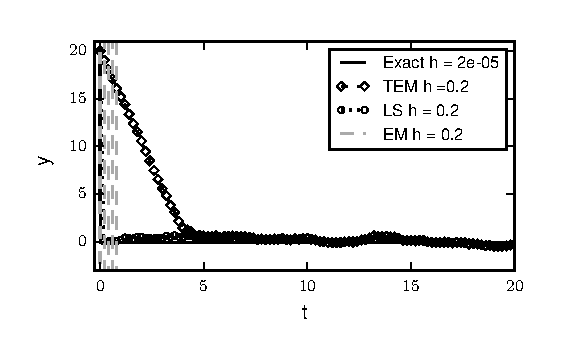
\includegraphics{papers/paperB/figures/ApplebyEx}
		\end{center}
		\caption{Likening between the EM, TEM and \SM approximations with unstable EM conditions. Here "exact" means
			a BEM solution with step size $h=\num{2e-5}$.}
		\label{fig:pathsAppleby}
	\end{figure}
\end{example}

\begin{example} We examine the \SM method using a SDE with super-linear grow diffusion. We 
	consider the SDE reported by \citeauthor*{Tretyakov2013} in \cite[Eq. (5.6)]{Tretyakov2013}
	\begin{equation}\label{eqn:SDETretyakov}
		dy(t) =
		\left(
			1-y^5(t) +y^3(t)  
		\right) dt
		+
		y^2(t) dW(t), \qquad y_0=0.
	\end{equation}
	\citeauthor{Tretyakov2013} show via simulation of \eqref{eqn:SDETretyakov} that the increment-tamed scheme
	\cite[Eq(1.5)]{Hutzenthaler2015}
	\begin{equation}\label{eqn:Increment-Tamed}
		X_{k+1} = X_k + 
		\frac{
			f(X_k) h + 
			g(X_k)\Delta W_k 
		}{
		\max\left(
		1, h
		\left|
		h f(X_k) +
		g(X_k)\Delta W_k
		\right|
	\right)}
	\end{equation}
	produces spurious oscillations. \citeauthor{Hutzenthaler2015} prove the convergence of this scheme under
	linear growth condition over diffusion. So, this suggests us that only certain kind of 
	explicit schemes with convergence under globally Lipschitz and linear growth diffusion conditions	
	%globally Lipschitz diffusion and linear growth 
	can extended their convergence to a locally Lipschitz diffusion and other kind of growth bound.
	Using $a(x):= -x^4 +x^2$, $b: = 1$ and $E=\{-1,0,1\}$, we construct the \SM method
	\begin{equation}\label{eqn:TreyakovLSMethod}
		Y_{k+1} = \exp(ha(Y_k))Y_k + 
		\frac{\exp(ha(Y_k)) - 1}{a(Y_k)} \1{E^c}
		+h\1{E}
		+Y_k^2\Delta W_k. 		
	\end{equation}
	\Cref{fig:Tretyakov} shows the numerical solution of SDE \eqref{eqn:SDETretyakov} with the Increment-Tamed (I-TEM) 
	\eqref{eqn:Increment-Tamed}, \SM method \eqref{eqn:TreyakovLSMethod}, and the Tamed (TEM) scheme. 
	We consider the implicit Midpoint scheme \cite[Eq.(5.3)]{Tretyakov2013} with $h=\num{e-4}$ 	as reference.
	\begin{figure}[h!]
		\centering
		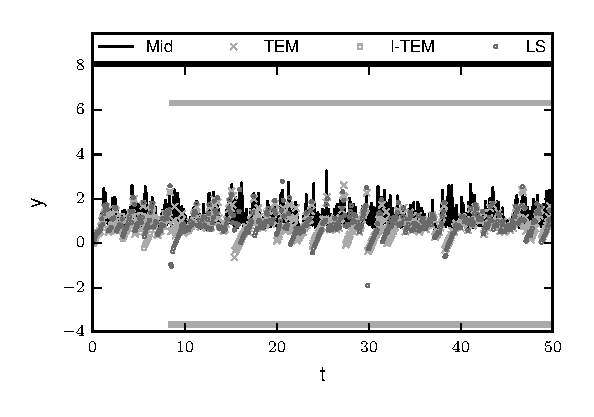
\includegraphics{./papers/paperB/figures/Tretyakov}
		\caption{
			Numerical solution of SDE \eqref{eqn:SDETretyakov} using the I-TEM 
			\eqref{eqn:Increment-Tamed}, \SM method \eqref{eqn:TreyakovLSMethod}  and TEM
			with $h=\num{0.1}$. The reference solution is a Midpoint rule approximation with $h=\num{e-4}$.
		}
		\label{fig:Tretyakov}
	\end{figure}
\end{example}

\begin{example}
	Now we compare the order of convergence and the run time of the \SM method with the TEM scheme as in 
	\cite{Hutzenthaler2012a}. That is, we consider a  Langevin equation under  the $d$-dimensional potential 
	$U(x)= \frac{1}{4}|x|^4 - \frac{1}{2}|x|^2$, and $d$-dimensional Brownian additive noise. The corresponding
	SDE reads
	\begin{equation}\label{eqn:SDELangevinHutz}
	dy(t) = 
		\left(
			y(t) - |y(t)| \cdot y(t)
		\right)dt
		+ dW(t), \qquad y(0)=0.
	\end{equation}
	This model describes the motion of a Brownian particle of unit mass immersed on the potential $U(x)$. 
	Taking $a_j(x):=1-|x|$ and $b_j=0$, $j\in \{1,\dots, d\}$ we obtain the \SM method
	\begin{equation}\label{eqn:LangevinLSMethod}
		Y_{k+1} = \diag
		\left[		
			e^{h a_1(Y_k)}, \dots, e^{ha_d(Y_k)}) 
		\right] 
		Y_k+
		\Delta W_k.
	\end{equation}
	\Cref{tbl:OrdersLS} shows the root means square errors at a final time $T=1$, which is approximated by
	\begin{equation}
		\sqrt{\EX{|Y_N - y(T)|^2}} \approx 
		\frac{1}{M}
		\left(
		\sum_{i=1}^M
		|y_i(T) - Y_{N,i}|^2	
		\right)^{1/2},
	\end{equation}
	over a sample of $M$ =\num{10000} trajectories of the TEM, \SM  and BEM solutions to SDE 
	\eqref{eqn:SDELangevinHutz} with dimension $d=10$.  We consider the TEM solution with step $h=2^{-19}$ as reference 
	solution. 
	In this experiment we confirm that the \SM method converges with standard order 1/2  and is almost equal accurate 
	as the TEM approximation.

		In some applicationa as in Browninan Dynamics Simulations \cite{Cruz2012}, the dimension of a SDE
	increases considerable the complexity and computational cost --- this excludes the use of implicit methods.
	In \Cref{fig:TimeVsDimension}, we observe that the runtime of the BEM method grows quadratically depending
	on the dimension, meanwhile the LS and TEM methods grow linearly. 
	\begin{table}[t]
		\centering
		\begin{tabular}{lllllll}
			&        TEM &        	& LS		&           & BEM		 &         \\
			\toprule
			h		& ms-error	 & ECO 		& ms-error	    & ECO		& ms-error	 &	ECO	  \\
			\midrule
			$2^{-2}$	& \num{1.70388}    & ---		&\num{1.55394}		& ---		& \num{1.38157}	& 
			--- \\
			$2^{-3}$	& \num{1.16977}    & \num{0.54}     &\num{1.10775}    & \num{0.48} & \num{1.05309}	& 
			\num{0.39} \\ 
			$2^{-7}$	&\num{0.27895}     & \num{0.48} & \num{0.27795}   & \num{0.48} & \num{0.276895}& 
			\num{0.48} \\
			$2^{-11}$	& \num{0.07010}  & \num{0.50} & \num{0.07009}  & \num{0.50} & \num{0.07007} & 
			\num{0.50} \\
			$2^{-15}$	& \num{0.01739}  & \num{0.51} & \num{0.01739}  & \num{0.51} & \num{0.01739}& 
			\num{0.51} \\
			\bottomrule
		\end{tabular}
		\caption{
			Mean square errors and the experimental convergence order (ECO) for the SDE \eqref{eqn:SDELangevinHutz} 
			with a TEM with $h = 2^{-19}$ as reference solution.
		}\label{tbl:OrdersLS}
	\end{table}
	\begin{figure}[t]
		\centering
			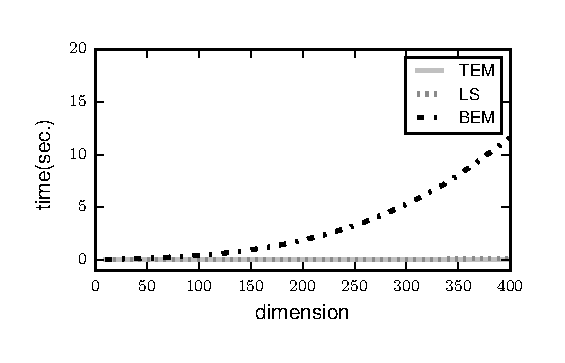
\includegraphics{./papers/paperB/figures/TimeVsDimension}
		\caption{
			Runtime calculation of $Y_N$ with $h=2^{-17}$, using the BEM,  \SM and TEM methods for 
			SDE \eqref{eqn:SDELangevinHutz}.
		}
		\label{fig:TimeVsDimension}
	\end{figure}
\end{example}

\begin{example}
	Let us recall the following  stochastic model for internal 
	HIV dynamics given by  \citeauthor{Dalal2008} in \cite{Dalal2008}:
	\begin{align}\label{eqn:StochasticHIVDynamics}
		dy_1(t) &=
		\left(
			\lambda -\delta y_1(t) - (1 - \gamma) \beta y_1(t) y_3(t)
		\right)dt
		-\sigma_1 y_1(t) dW^{(1)}_t, 
		\notag \\
		dy_2(t) &= 	
		\left(
			(1- \gamma) \beta y_1(t) y_3(t) - \alpha y_2(t) 
		\right)dt
		-\sigma_1 y_2(t) dW^{(1)}_t, 
		\\
		dy_3(t) & = 
		\left(
			(1 - \eta) N_0 \alpha y_2(t) 
				-\mu y_3(t)
			-(1 - \gamma ) \beta y_1(t) y_3(t) 
		\right)dt
		- \sigma_2 y_3(t) dW^{(2)}_t.
		\notag
	\end{align}	
	\begin{figure}[h!]
		\centering
		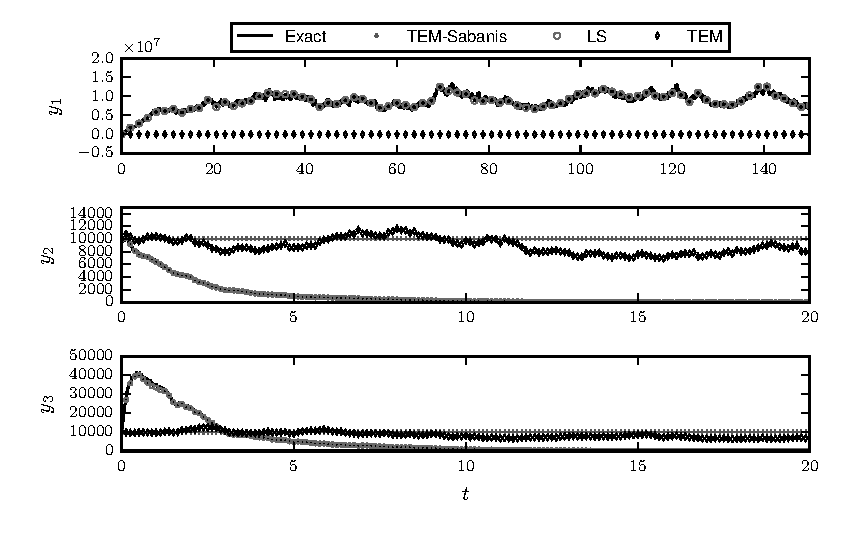
\includegraphics{./papers/paperB/figures/InternalHIVDynamics}
		\caption{
			Likening between EM, \SM, TEM approximations for SDE \eqref{eqn:StochasticHIVDynamics} with
			$\gamma = \num{0.5}$,
			$\eta = \num{0.5}$,
			$\lambda = \num{e6}$, 
			$\delta = \num{0.1}$,
			$\beta = \num{e-8}$,
			$\alpha = \num{0.5}$,
			$N_0= \num{100}$,
			$\mu = \num{5}$,
			$\sigma_1 = \num{0.1}$,
			$\sigma_2 = \num{0.1} $,
			$y_0 = (
			\num{10000},%{\per\cubic\deci\meter}, 
			\num{10000},%{\per\cubic\deci\meter}, 
			\num{10000}.%{\per\cubic\deci\meter}
			)^T$,
			$h=\num{0.125}$.
			Here the reference solution means a BEM simulation
			with the same parameters but with a step-size $h=\num{e-5}$.
		}
		\label{fig:InternalHIVDynamics5e-1}
	\end{figure} 
	Under certain conditions \citeauthor{Dalal2008} prove 
	that  system \eqref{eqn:StochasticHIVDynamics} has a unique 
	almost surely exponential stability solution, that is,  $y=(y_1,y_2,y_3)$  tends 
	exponentially to an equilibrium $(\bar{y}_1,0,0)$ with probability 1. 
	Now, we want to verify if  the EM, TEM, TEM-Sabanis \cite{Sabanis2015} and LS approximations can reproduce this 
	property of the solution. Taking 
	\begin{align*}
		E_1&:=\left\{
			(x,y,z)^T \in \R^3:
			z=0 
			\text{ or }
			z=0
			\frac{-\delta}{\beta(1-\gamma)}
		\right\}, \quad
		E_2:=	\emptyset,   \\
		E_3&:=\left\{
			(x,y,z)^T \in \R^3: 
			x=0
			\text{ or }
			x=
			\frac{-\mu}{\beta(1-\gamma)}
		\right\}
	\end{align*}
	 
	The LS method for \eqref{eqn:StochasticHIVDynamics} is given by
	
	\begin{align}
		a_{1}(Y_k)) &:= 
		-\left(
		\delta + (1 - \gamma) \beta Y_k^{(3)}
		\right),		
		& b_1(Y_k^{(-1)}) &:= \lambda, 
		& 
		\notag
		\\
		a_{2}(Y_k) &:= -\alpha,
		&b_2(Y_k^{(-2)}) & :=
		(1-\gamma) \beta Y_{k}^{(1)} Y_{k}^{(3)},
		\notag
		\\
		a_{3}(Y_k) &= 
		-
		\left(
		\mu + (1- \gamma) \beta Y_{k}^{(1)}
		\right),
		\qquad
		%
		&b_{3}(Y_k^{(-3)}) &:= 
		\left(
		1 - \eta 
		\right)
		N_0 \alpha Y_{k}^{(2)},
		\notag			
	\end{align}
	the \SM method for the stochastic model \eqref{eqn:StochasticHIVDynamics} reads,
	\begin{align}
		Y_{k+1} &= A^{(1)}(h,Y_k) \,Y_k + A^{(2)}(h,Y_k)b(Y_k)+ g(Y_k)\, \Delta W_k,
		\qquad \Delta W_k = \left(W_k^{(1)}, W_k^{(2)}\right)^T, 
		\notag\\ 
		A^{(1)}(h,Y_k)&:=
		\begin{pmatrix}
			e^{ha_1(Y_k)}	&	0	&0 \\
			0	&e^{ha_2(Y_k))}	&0\\
			0	&0				&e^{ha_3(Y_k))}
		\end{pmatrix},
		%	
		\notag
		\\
		%	
		A^{(2)}&:=
		\begin{pmatrix}
			h \Phi_1(Y_k)\1{E_1^c}	&0	&0\\
			0 & 
			\left(\displaystyle
			\frac{e^{-h\alpha} - 1}{\alpha}
			\right) & 0\\
			0 & 0 & h \Phi_3(Y_k)\1{E_3^c} 
		\end{pmatrix}
		%\notag \\
		+h
		\begin{pmatrix}
			\1{E_1}	&0 			&0\\
			0		&0			&0\\
			0		&0			&\1{E_3}\\
		\end{pmatrix},
	\notag
	\\
	b(Y_k) &:=
	\begin{pmatrix}
		b_1(Y_k^{(-1)})\\
		b_2(Y_k^{(-2)})\\
		b_3(Y_k^{(-3)})
	\end{pmatrix},
	\qquad
	g(Y_k):=
	\begin{pmatrix}
		-\sigma_1 Y_k^{(1)}	&0\\
		-\sigma_1 Y_k^{(2)}	&0\\
		0	&-\sigma_2 Y_k^{(3)}
	\end{pmatrix}.
\end{align}
%
	\Cref{fig:InternalHIVDynamics5e-1} shows the  \SM, TEM and TEM-Sabanis approximations
	with the parameters reported in \cite{Dalal2008}.  The EM approximation
	blows up  so it is not drawn. We observe how the TEM approximation (components $y_2$ and $y_3$) oscillates about 
	the initial condition and the 
	TEM-Sabanis approximation (components $y_2$ and $y_3$) is constant and equal to the initial value, while the \SM 
	method reproduces the asymptotic behaviour of the solution. It is important to remark that the Tamed family methods	
	improve convergence of the Euler method by taming the drift increment term with 
	the factor	$1/(1 + h |f(Y_k)|)$, bounding the norm of  $h f(Y_k)/(1 + h |f(Y_k)|)$ by 1. This norm   
	controls the drift contribution of the Tamed methods  at each step. Such modification 
	is recommended for SDEs with drift contributions and initial conditions with similar scales. We observe
	that for models where such terms have different scales the TEM over damps the drift contribution. 
\end{example}


	%\section{Almost sure Stability}
		%	In this section we study the globally almost surely asymptotic stability (as-stability) of the 
Linear Steklov  method \crefrange{eqn:SSLSM1}{eqn:SSLSM2}, in the scalar case.
For simplicity we assume that the drift coefficient satisfies
$$
	f(x) = a(x)x,
$$
for some suitable nonlinear function $a:\R \to \R$.
Here, we will follow the same technique reported by \citeauthor*{Mao2013} in \cite{Mao2013}.
First, we need sufficient conditions to characterize when the solution of the SDE \eqref{eqn:SDE1} is as-stable. 
The following result deals with it.

\begin{thm}[Mao and Szpruch {\cite[Thm. 2.2]{Mao2013}}]
	Let \cref{ass:OSLC} hold and suppose that there exists a function $z\in \mathcal{C}(\mathbb{R}^d,\mathbb{R}_+)$
	such that
	\begin{equation*}
		\innerprod{x}{f(x)} +
		\frac{1}{2}|g(x)|^2\leq -z(x), \qquad \forall x\in \mathbb{R}^d,
	\end{equation*}
	then 
	\begin{enumerate}[(i)]
		\item
			For any $y_0\in \mathbb{R}^n$ the solution of the SDE \eqref{eqn:SDE1}, $y(t)$, satisfies
			\begin{equation*}
				\limsup_{t\to \infty}
					|y(t)|^2 \leq \infty \qquad \as \qquad \text{and} \qquad 
					\lim_{t\to \infty} z(y(t))= 0 \qquad \as
			\end{equation*}
		\item
			additionally, if $z(x)=0$ only when it is evaluated at $x=0$, then
			\begin{equation*}
				\lim_{t\to \infty} y(t)=0 \qquad \as \qquad \forall y_0\in \R^d.
			\end{equation*}
	\end{enumerate}
\end{thm}

	Next, %in\Cref{thm:AlmosSurleyStability}
we prove that \SM method verifies the as-stability.
The proof of this result depends on the \Cref{lem:MartingaleConvergence} see for instance 
\cite[Th. 7, pg. 139]{Liptser1989}.
We will denote by  $\{Z\to\}$ the set of all $\omega \in \Omega$ for which the scalar process $Z$ has the property that
$\lim_{k\to\infty} Z_k$ exists and is finite.
\begin{lem}[{\cite[Thm. 7, pg. 139]{Liptser1989}}]
	\label{lem:MartingaleConvergence}
	Let $Z= \{Z_k\}$ be a nonnegative semimartingale with $\mathbb{E}|Z|<\infty$ and Doob decomposition 
	$$
		Z = Z_0 + A^{(1)} -A^{(2)} + M,
	$$
	where 
	$A^{(1)}:=\{A_k^{(1)}\}_{k\in \N}$ and $A^{(2)}:=\{A_k^{(2)}\}_{k\in \N}$ are $\as$ nondecreasing predictable
	processes with $A_0^{(1)}=A_0^{(2)}=0$ and $M:=\{M_k\}_{k\in\N}$ is a local $\{\calF_k\}$-martingale with $M_0=0$.
	Then
	\begin{equation*}
		\left\{
			%\omega:
			%\lim_{n\to \infty}
				A^{(1)} \to
		\right\}
		\subseteq
		\left\{
			%\omega:
			%\lim_{n\to \infty}
				A^{(2)} \to
		\right\}\cap
		\left\{
			%\lim_{n\to \infty}
			Z \to
		\right\} \qquad \as
\end{equation*}
\end{lem}
\begin{thm}\label{thm:AlmosSurleyStability}
		Let \Cref{ass:OSLC} hold. Suppose that there is a function 
		$z \in \calC(\R^n,\R_+)$ 
		and a step size $h^*>0$ such that for all $x\in \R$ and for all $h$ in $(0,h^*)$,
		\begin{align} 
			\innerprod{x}{f(x)} + \frac{1}{2}|g(x)|^2
			&\leq -z(x), \label{eqn:ConditionStability1}\\
			|x|^2
			\frac{(\exp(2 h a(x))-1)}{h}
			+|g_h(x)|^2
			&\leq
				-z(x), \label{eqn:ConditionStability2}
		\end{align}
	Then the \SM method defined by \crefrange{eqn:SSLSM1}{eqn:SSLSM2} satisfies
	\begin{align*}
		\limsup_{k\to \infty}
			|Y_k|^2 
			& <\infty \quad\text{ and} 
			\quad
		\lim_{k\to \infty}
			w(Y_k) =0. 
	\end{align*}
In addition, if $z(x)=0$ only when $x=0$, then
	$ \displaystyle
		\lim_{k\to \infty} Y_k = 0.
	$
\end{thm}
\begin{proof}
	Taking advantage of \Cref{lem:MartingaleConvergence}, we proceed to construct a conveniently 
	semimartingale. To
	\begin{align}
		|Y_{k+1}|^2
			&=
				|Y_{k}|^2
				+h^2|\varphi_{f_h}(Y_{k})|^2 
				+|g_h(Y_k) \Delta W_k|^2 \notag 
				+2h\innerprod{Y_k}{\varphi_{f_h}(Y_{k})} 
				\notag\\
			%
			&
				+2\innerprod{Y_k}{g_h(Y_{k})\Delta W_k}
				+2h\innerprod{\varphi_{f_h}(Y_{k})}{g_h(Y_{k})\Delta W_k}.
			\label{eqn:ExpandOfYnext}
	\end{align}
	Let 
	\begin{align*}
		\Delta M_{k+1}
			&:=
				|g_h(Y_k)\Delta W_{k+1}|^2 - |g_h(Y_k)|^2 h \notag \\
			&
			+2\innerprod{Y_k}{g_h(Y_{k})\Delta W_{k+1}}
			+2h\innerprod{\varphi_{f_h}(Y_{k})}{g_h(Y_{k})\Delta W_{k+1}}, \notag
	\end{align*}
	which is a local martingale.
	Taking
	$ %\begin{equation}\label{eqn:BjNotation}
		B_j:=
			-\left[
					2\innerprod{Y_j}{\varphi_{f_h}(Y_j)}
					+|g_h(Y_j)|^2
				+h|\varphi_{f_h}(Y_j)|^2
			\right],
	$ %\end{equation}
	and fixing $N\in \N$, we can rewrite \eqref{eqn:ExpandOfYnext} as
	\begin{align}\label{eqn:MartingaleDecomposition}
		|Y_{N+1}|^2 = 
			|Y_0|^2
				-\sum_{j=0}^{N} B_j h
				+\sum_{j=0}^{N} \Delta M_{j+1}.
	\end{align} 
	To prove that \eqref{eqn:MartingaleDecomposition} is the required decomposition to apply
	\Cref{lem:MartingaleConvergence}, we use that
	\begin{equation}\label{eqn:varphih(x)}
		\varphi_{f_h}(x)
			= x\frac{\left(\exp(h a(x))-1\right)}{h}.
	\end{equation}
	By algebraic manipulations, we obtain
	\begin{equation*}
		B_j=
		-\left[
			|Y_j|^2\frac{(\exp(2h a(Y_j))-1)}{h}
			+|g_h(Y_j)|^2
		\right],
		%\geq z(Y_j) \geq 0,
		\qquad
		 j=0,\dots,N.
	\end{equation*}
	Given that inequality \eqref{eqn:ConditionStability2} holds, we can deduce that
	$$
		B_j\geq z(Y_j) \geq 0, \quad j=0,\ldots N.
	$$
	Consequently, $A_k^{(2)}:=\sum_{j=0}^k B_jh$ is a non decreasing process.
	Finally, taking $A^{(1)}=0$,  $Z=|Y_k|^2$ and $M_k=\sum_{j=0}^k \Delta M_{j+1}$.
	We can deduce  by \Cref{lem:MartingaleConvergence} that $\{A^{(1)}\to\}=\Omega$, thus
	\begin{align*}
	 \limsup_{k\to \infty}
			|Y_k|^2 < \infty \quad \as,
		\quad \text{and} \quad
		\sum_{j=0}^\infty z(Y_k) 
		\leq 
		\sum_{j=0}^\infty B_jh < \infty.
	\end{align*}
	Consequently
	$
		%\displaystyle
		\lim_{k\to \infty} z(Y_k) =0
	$,
	and the theorem follows.
\end{proof}
%

	%		In this section we study the globally almost surely asymptotic stability (as-stability) of the 
Linear Steklov  method \crefrange{eqn:SSLSM1}{eqn:SSLSM2}, in the scalar case.
For simplicity we assume that the drift coefficient satisfies
$$
	f(x) = a(x)x,
$$
for some suitable nonlinear function $a:\R \to \R$.
Here, we will follow the same technique reported by \citeauthor*{Mao2013} in \cite{Mao2013}.
First, we need sufficient conditions to characterize when the solution of the SDE \eqref{eqn:SDE1} is as-stable. 
The following result deals with it.

\begin{thm}[Mao and Szpruch {\cite[Thm. 2.2]{Mao2013}}]
	Let \cref{ass:OSLC} hold and suppose that there exists a function $z\in \mathcal{C}(\mathbb{R}^d,\mathbb{R}_+)$
	such that
	\begin{equation*}
		\innerprod{x}{f(x)} +
		\frac{1}{2}|g(x)|^2\leq -z(x), \qquad \forall x\in \mathbb{R}^d,
	\end{equation*}
	then 
	\begin{enumerate}[(i)]
		\item
			For any $y_0\in \mathbb{R}^n$ the solution of the SDE \eqref{eqn:SDE1}, $y(t)$, satisfies
			\begin{equation*}
				\limsup_{t\to \infty}
					|y(t)|^2 \leq \infty \qquad \as \qquad \text{and} \qquad 
					\lim_{t\to \infty} z(y(t))= 0 \qquad \as
			\end{equation*}
		\item
			additionally, if $z(x)=0$ only when it is evaluated at $x=0$, then
			\begin{equation*}
				\lim_{t\to \infty} y(t)=0 \qquad \as \qquad \forall y_0\in \R^d.
			\end{equation*}
	\end{enumerate}
\end{thm}

	Next, %in\Cref{thm:AlmosSurleyStability}
we prove that \SM method verifies the as-stability.
The proof of this result depends on the \Cref{lem:MartingaleConvergence} see for instance 
\cite[Th. 7, pg. 139]{Liptser1989}.
We will denote by  $\{Z\to\}$ the set of all $\omega \in \Omega$ for which the scalar process $Z$ has the property that
$\lim_{k\to\infty} Z_k$ exists and is finite.
\begin{lem}[{\cite[Thm. 7, pg. 139]{Liptser1989}}]
	\label{lem:MartingaleConvergence}
	Let $Z= \{Z_k\}$ be a nonnegative semimartingale with $\mathbb{E}|Z|<\infty$ and Doob decomposition 
	$$
		Z = Z_0 + A^{(1)} -A^{(2)} + M,
	$$
	where 
	$A^{(1)}:=\{A_k^{(1)}\}_{k\in \N}$ and $A^{(2)}:=\{A_k^{(2)}\}_{k\in \N}$ are $\as$ nondecreasing predictable
	processes with $A_0^{(1)}=A_0^{(2)}=0$ and $M:=\{M_k\}_{k\in\N}$ is a local $\{\calF_k\}$-martingale with $M_0=0$.
	Then
	\begin{equation*}
		\left\{
			%\omega:
			%\lim_{n\to \infty}
				A^{(1)} \to
		\right\}
		\subseteq
		\left\{
			%\omega:
			%\lim_{n\to \infty}
				A^{(2)} \to
		\right\}\cap
		\left\{
			%\lim_{n\to \infty}
			Z \to
		\right\} \qquad \as
\end{equation*}
\end{lem}
\begin{thm}\label{thm:AlmosSurleyStability}
		Let \Cref{ass:OSLC} hold. Suppose that there is a function 
		$z \in \calC(\R^n,\R_+)$ 
		and a step size $h^*>0$ such that for all $x\in \R$ and for all $h$ in $(0,h^*)$,
		\begin{align} 
			\innerprod{x}{f(x)} + \frac{1}{2}|g(x)|^2
			&\leq -z(x), \label{eqn:ConditionStability1}\\
			|x|^2
			\frac{(\exp(2 h a(x))-1)}{h}
			+|g_h(x)|^2
			&\leq
				-z(x), \label{eqn:ConditionStability2}
		\end{align}
	Then the \SM method defined by \crefrange{eqn:SSLSM1}{eqn:SSLSM2} satisfies
	\begin{align*}
		\limsup_{k\to \infty}
			|Y_k|^2 
			& <\infty \quad\text{ and} 
			\quad
		\lim_{k\to \infty}
			w(Y_k) =0. 
	\end{align*}
In addition, if $z(x)=0$ only when $x=0$, then
	$ \displaystyle
		\lim_{k\to \infty} Y_k = 0.
	$
\end{thm}
\begin{proof}
	Taking advantage of \Cref{lem:MartingaleConvergence}, we proceed to construct a conveniently 
	semimartingale. To
	\begin{align}
		|Y_{k+1}|^2
			&=
				|Y_{k}|^2
				+h^2|\varphi_{f_h}(Y_{k})|^2 
				+|g_h(Y_k) \Delta W_k|^2 \notag 
				+2h\innerprod{Y_k}{\varphi_{f_h}(Y_{k})} 
				\notag\\
			%
			&
				+2\innerprod{Y_k}{g_h(Y_{k})\Delta W_k}
				+2h\innerprod{\varphi_{f_h}(Y_{k})}{g_h(Y_{k})\Delta W_k}.
			\label{eqn:ExpandOfYnext}
	\end{align}
	Let 
	\begin{align*}
		\Delta M_{k+1}
			&:=
				|g_h(Y_k)\Delta W_{k+1}|^2 - |g_h(Y_k)|^2 h \notag \\
			&
			+2\innerprod{Y_k}{g_h(Y_{k})\Delta W_{k+1}}
			+2h\innerprod{\varphi_{f_h}(Y_{k})}{g_h(Y_{k})\Delta W_{k+1}}, \notag
	\end{align*}
	which is a local martingale.
	Taking
	$ %\begin{equation}\label{eqn:BjNotation}
		B_j:=
			-\left[
					2\innerprod{Y_j}{\varphi_{f_h}(Y_j)}
					+|g_h(Y_j)|^2
				+h|\varphi_{f_h}(Y_j)|^2
			\right],
	$ %\end{equation}
	and fixing $N\in \N$, we can rewrite \eqref{eqn:ExpandOfYnext} as
	\begin{align}\label{eqn:MartingaleDecomposition}
		|Y_{N+1}|^2 = 
			|Y_0|^2
				-\sum_{j=0}^{N} B_j h
				+\sum_{j=0}^{N} \Delta M_{j+1}.
	\end{align} 
	To prove that \eqref{eqn:MartingaleDecomposition} is the required decomposition to apply
	\Cref{lem:MartingaleConvergence}, we use that
	\begin{equation}\label{eqn:varphih(x)}
		\varphi_{f_h}(x)
			= x\frac{\left(\exp(h a(x))-1\right)}{h}.
	\end{equation}
	By algebraic manipulations, we obtain
	\begin{equation*}
		B_j=
		-\left[
			|Y_j|^2\frac{(\exp(2h a(Y_j))-1)}{h}
			+|g_h(Y_j)|^2
		\right],
		%\geq z(Y_j) \geq 0,
		\qquad
		 j=0,\dots,N.
	\end{equation*}
	Given that inequality \eqref{eqn:ConditionStability2} holds, we can deduce that
	$$
		B_j\geq z(Y_j) \geq 0, \quad j=0,\ldots N.
	$$
	Consequently, $A_k^{(2)}:=\sum_{j=0}^k B_jh$ is a non decreasing process.
	Finally, taking $A^{(1)}=0$,  $Z=|Y_k|^2$ and $M_k=\sum_{j=0}^k \Delta M_{j+1}$.
	We can deduce  by \Cref{lem:MartingaleConvergence} that $\{A^{(1)}\to\}=\Omega$, thus
	\begin{align*}
	 \limsup_{k\to \infty}
			|Y_k|^2 < \infty \quad \as,
		\quad \text{and} \quad
		\sum_{j=0}^\infty z(Y_k) 
		\leq 
		\sum_{j=0}^\infty B_jh < \infty.
	\end{align*}
	Consequently
	$
		%\displaystyle
		\lim_{k\to \infty} z(Y_k) =0
	$,
	and the theorem follows.
\end{proof}
%

			%		\todo{Put here the stochastic extension of the Bone Remodeling model.}
	\pagebreak
	\section*{\refname}
	\bibliographystyle{plainnat}
	\bibliography{bib/PhdThesisBib}
\appendix
	\begin{appendices}
		\section{Useful Inequalities}
			\begin{Holder}
	\begin{equation}\label{eqn:HolderInequality}
	\m[X^T Y] \leq
	\left(
	\m|X|^p
	\right)^{\frac{1}{p}}		
	\left(
	\m|X|^q
	\right)^{\frac{1}{q}}.
	\end{equation}
\end{Holder}

\begin{Young}
	\begin{equation}\label{eqn:YoungsInequality}
	|a||b| 
	\leq
	\frac{\delta}{p} |a|^p
	+\frac{\delta}{q \delta^{q/p}} |b|^q.
	\end{equation}
\end{Young}
%
\begin{Minkowski}
	\begin{equation}
	\left(
	\m |X+Y|^p
	\right)^{\frac{1}{p}}
	\leq
	\left(
	\m |X|^p
	\right)^{\frac{1}{p}}
	+
	\left(
	\m |Y|^p
	\right)^{\frac{1}{p}}.
	\end{equation}
\end{Minkowski}
%
%
\begin{Standard}
		Fix $1<p<\infty$ and consider a sequence of real numbers $\{a_i\}_{i=1}^{N}$  with $N \in \N$. Then one can 
	formulate this usefully inequality
	\begin{equation}\label{eqn:SingleHolder}
	\left(
	\sum_{j=1}^N a_j
	\right)^p
	\leq
	N^{p-1}
	\sum_{j=1}^{N}
	a_j^p.
	\end{equation}
\end{Standard}
%
\begin{Doobs}
%\begin{thm}[Doob's Martingale Inequality]
	Let $\{M_t\}_{t\geq 0}$ be a $\mathbb{R}^d$-valued martingale. Let $[a,b]$ be a bounded interval in $
	\mathbb{R}_{+}$.
	If $p>1$ and $M_t\in L^p(\Omega;\mathbb{R}^d)$ then
	\begin{equation}
	\label{eqn:DoobMartingaleInequality}
	\m\left( \sup_{a\leq t \leq b} |M_t|^p\right) 
	\leq \left(\frac{p}{p-1}\right)^p \m|M_b|^p. 
	\end{equation}
%\end{thm}
\end{Doobs}

\begin{bdg}
	Let $g\in \mathcal{L}(\mathbb{R}_+; \mathbb{R}^{d\times m})$. Define for $t\geq 0$
	\begin{equation}
		\label{thm:BDG}
		x(t) = \int_{0}^{t} g(s)dW(s) \quad \text{and } \qquad 
		A(t) = \int_{0}^{t} |g(s)|^2 ds.
	\end{equation}
	Then for all $p>0$, there exist universal positive constants $c_p$, $C_p$ such that
	\begin{equation}
		c_p\m|{A(t)}|^{\frac{p}{2}}
		\leq
		\m \left[
		\sup_{0\leq s \leq t} |x(s)|^p
		\right]
		\leq 
		C_p \m |A(t)|^{\frac{p}{2}},
	\end{equation}
	for all $t\geq 0$.  In particular, one may take
	\begin{align*}
	c_p &= (p/2)^p, & 			 C_p &= (32/p)^{\frac{p}{2}} & \text{if } 0<p<2; \\
	c_p &= 1,       & 			 C_p &= (32/p)^{\frac{p}{2}} & \text{if } p=2; \\
	c_p &= (2p)^{-\frac{p}{2}},& C_p &= \frac{p+1}{2(p-1)^{\frac{p}{2}}} & \text{if } p>2 .\\
	\end{align*}
\end{bdg}

\begin{Gronwall}
	Let $T > 0$ and $c \geq 0$. Let $u(\cdot)$ be a Borel measurable bounded nonnegative function on 
	$[0,T]$, and let $v$ be a nonnegative integrable function on $[0,T]$
	If
	$$
		u(t) \leq c 
		+\int_{0}^{t} v(s)u(s)ds \qquad \forall t \in [0,T],
	$$
	then
	\begin{equation}\label{thm:Gronwall}
		u(t) \leq c\exp
		\left(
		\int_{0}^{t} v(s)ds 
		\right)
		\qquad \forall t \in [0,T].
	\end{equation}
\end{Gronwall}
%
\begin{DiscreteGronwall}
	Let $M$ be a positive integer. Let $u_k$ and $v_k$ be non-negative numbers for $k=0,1,\dots,M$. 
	If
	$$
	u_k\leq u_0 + \sum_{j=0}^{k-1} u_j v_j
	$$
	then
	\begin{equation}
		\label{thm:DiscreteGronwall}
		u_k \leq u_0 
		\exp
		\left(
		\sum_{j=0}^{k-1}v_j
		\right).
	\end{equation}
\end{DiscreteGronwall}

	\end{appendices}
\end{document}
